%%%%%%%% ICML 2018 EXAMPLE LATEX SUBMISSION FILE %%%%%%%%%%%%%%%%%

\documentclass{article}

% Recommended, but optional, packages for figures and better typesetting:
\usepackage{microtype}
\usepackage{graphicx}
\usepackage{subfigure}
\usepackage{booktabs} % for professional tables

% hyperref makes hyperlinks in the resulting PDF.
% If your build breaks (sometimes temporarily if a hyperlink spans a page)
% please comment out the following usepackage line and replace
% \usepackage{icml2018} with \usepackage[nohyperref]{icml2018} above.
\usepackage{hyperref}

% Attempt to make hyperref and algorithmic work together better:
\newcommand{\theHalgorithm}{\arabic{algorithm}}

% Use the following line for the initial blind version submitted for review:
%\usepackage{icml2018}

% If accepted, instead use the following line for the camera-ready submission:
\usepackage[accepted]{icml2018}

% for code block
%\usepackage{listings}

% The \icmltitle you define below is probably too long as a header.
% Therefore, a short form for the running title is supplied here:
\icmltitlerunning{World Models}



% Chinese translation support
\usepackage{xeCJK}
\setCJKmainfont{FandolSong-Regular.otf}[ItalicFont=FandolKai-Regular.otf]
\setCJKsansfont{FandolHei-Regular.otf}
\setCJKmonofont{FandolFang-Regular.otf}
\XeTeXlinebreaklocale "zh"
\XeTeXlinebreakskip = 0pt plus 1pt
\renewcommand{\abstractname}{摘要}
\renewcommand{\figurename}{图}
\renewcommand{\tablename}{表}
\makeatletter
\@ifundefined{captionsetup}{}{%
 \captionsetup[figure]{name=图}%
 \captionsetup[table]{name=表}%
}
\renewcommand{\fnum@figure}{图~\thefigure}
\renewcommand{\fnum@table}{表~\thetable}
\makeatother
\renewcommand{\refname}{参考文献}
\renewcommand{\contentsname}{目录}
\renewenvironment{abstract}
   {%
\centerline{\large\bf 摘要}
    \vspace{-0.12in}\begin{quote}}
   {\par\end{quote}\vskip 0.12in}
\makeatletter
\AtBeginDocument{%
 \@ifundefined{crefname}{}{%
 \crefname{figure}{图}{图}%
 \Crefname{figure}{图}{图}%
 \crefname{table}{表}{表}%
 \Crefname{table}{表}{表}%
 \crefname{section}{节}{节}%
 \Crefname{section}{节}{节}%
 \crefname{appendix}{附录}{附录}%
 \Crefname{appendix}{附录}{附录}%
 \crefname{algocf}{算法}{算法}%
 \Crefname{algocf}{算法}{算法}%
 }%
 \@ifundefined{SetAlgorithmName}{}{\SetAlgorithmName{算法}{算法}{算法列表}}%
}
\makeatother
\raggedbottom

\begin{document}

\twocolumn[
\icmltitle{World Models}

% It is OKAY to include author information, even for blind
% submissions: the style file will automatically remove it for you
% unless you've provided the [accepted] option to the icml2018
% package.

% List of affiliations: The first argument should be a (short)
% identifier you will use later to specify author affiliations
% Academic affiliations should list Department, University, City, Region, Country
% Industry affiliations should list Company, City, Region, Country

% You can specify symbols, otherwise they are numbered in order.
% Ideally, you should not use this facility. Affiliations will be numbered
% in order of appearance and this is the preferred way.
\icmlsetsymbol{equal}{*}

\begin{icmlauthorlist}
\icmlauthor{David Ha}{goo}
\icmlauthor{J\"{u}rgen Schmidhuber}{nnaisense,idsia}
\end{icmlauthorlist}

%\author{J\"{u}rgen Schmidhuber~\\
%NNAISENSE, Lugano, Switzerland \\
%The Swiss AI Lab, IDSIA \\
%Istituto Dalle Molle di Studi sull'Intelligenza Artificiale \\
%Scuola universitaria professionale della Svizzera italiana \\
%Universit\`{a} della Svizzera italiana, Switzerland
%}

%here is the maximally compressed form:
%1. NNAISENSE
%2. Swiss AI Lab, IDSIA (USI & SUPSI)

\icmlaffiliation{goo}{\scriptsize Google Brain}
\icmlaffiliation{nnaisense}{\scriptsize NNAISENSE}
\icmlaffiliation{idsia}{\scriptsize Swiss AI Lab, IDSIA (USI \& SUPSI)}

%\icmlcorrespondingauthor{David Ha}{hadavid@google.com}

% You may provide any keywords that you
% find helpful for describing your paper; these are used to populate
% the "keywords" metadata in the PDF but will not be shown in the document
\icmlkeywords{Machine Learning}

\vskip 0.3in
]
% this must go after the closing bracket ] following \twocolumn[ ...

% This command actually creates the footnote in the first column
% listing the affiliations and the copyright notice.
% The command takes one argument, which is text to display at the start of the footnote.
% The \icmlEqualContribution command is standard text for equal contribution.
% Remove it (just {}) if you do not need this facility.

\printAffiliationsAndNotice{} % leave blank if no need to mention equal contribution

\begin{abstract}
我们探索为常见强化学习环境构建生成式神经网络模型。\textit{世界模型} 可以通过无监督方式快速训练，学习环境在空间和时间上的压缩表示。将世界模型提取的特征作为智能体输入后，我们可以训练一个非常紧凑、结构简单的策略来完成目标任务。甚至可以让智能体完全在自己的世界模型生成的“幻觉梦境”中训练，再把学到的策略迁移回真实环境。\\ \\ 本文的交互式版本见：\url{https://worldmodels.github.io}
\end{abstract}

\section{导言}
\label{introduction}

人类会根据有限的感官输入形成关于世界的心理模型，并在这个内部模型的基础上作出决定和采取行动。系统动力学奠基人 Jay Wright Forrester 曾这样描述心理模型:

\textit{我们头脑中的世界图像只是一个模型。没有人能在头脑中容纳整个世界、政府或国家；他只能选择若干概念及其关系，并用它们来代表真实系统。}~\cite{forrester}

\begin{figure}[ht]
\vskip -0.0in
\begin{center}
\centerline{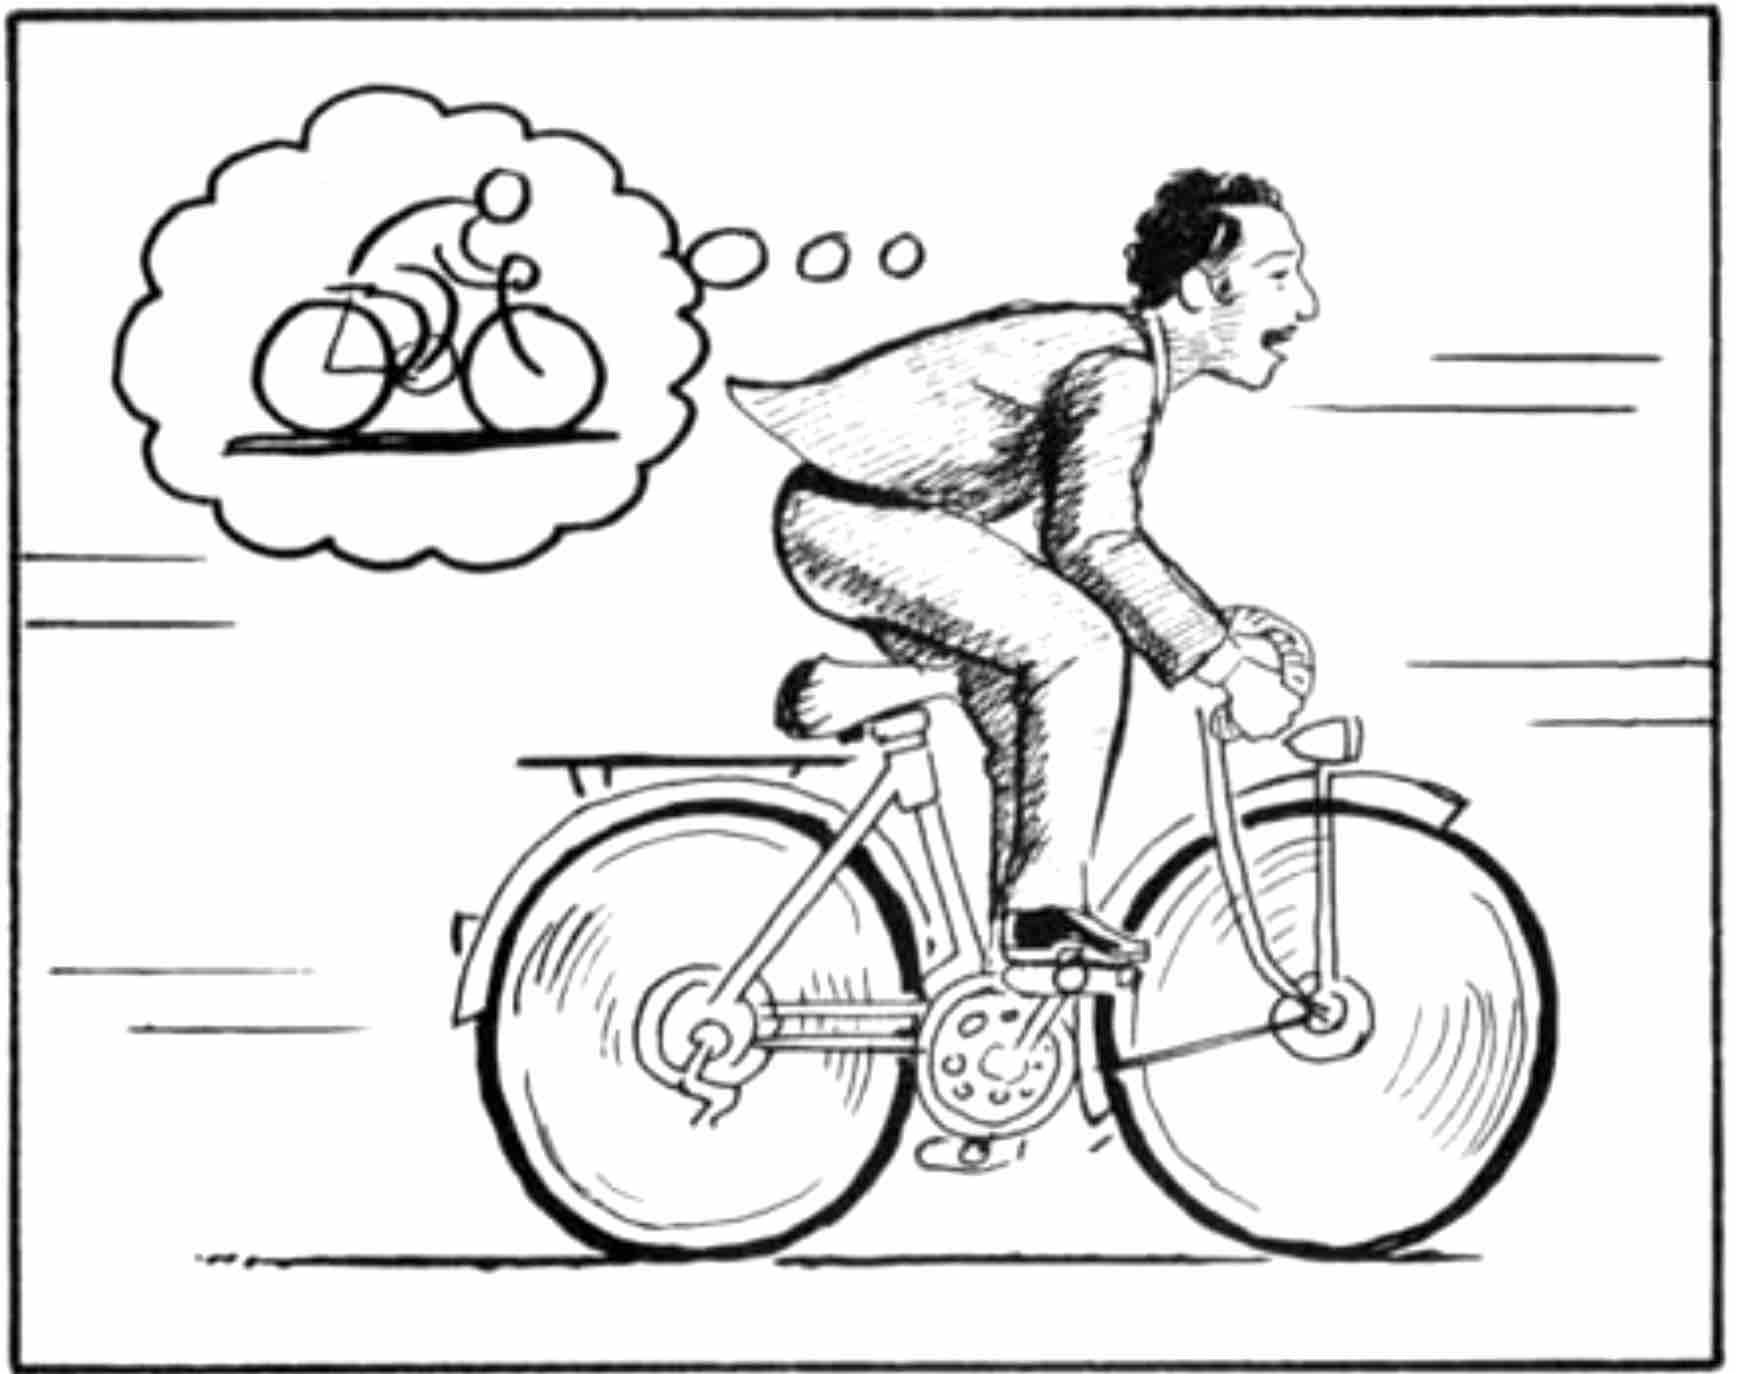
\includegraphics[width=0.9\columnwidth]{assets/world_model_comic.jpeg}}
\vskip -0.10in
\caption{来自 Scott McCloud \textit{Understanding Comics} 的 “A World Model”~\cite{understandingcomics,understandingcomics_blog}。}
\label{understanding_comics_figure}
\end{center}
\vskip -0.45in
\end{figure}

为了处理日常生活中涌入的大量信息，大脑会学习这些信息在空间和时间上的抽象表示。我们能够观察一个场景，并记住对它的抽象描述\cite{facial_identity_primate_brain,single_neuron_viz}。证据也表明，我们在任一时刻的感知并非只由当前输入决定，还受到大脑内部模型对未来的预测影响\cite{primary_viz_cortex_past_present,mt_motion}。

理解大脑内部预测模型的一种方式是：它并非笼统地预测未来，而是在给定当前运动动作的情况下预测未来的感官数据\cite{Keller2012,Leinweber2017}。当面临危险时，我们能够直接基于这种预测模型作出快速反射行为\cite{survival_optimization}，不必有意识地规划完整的动作序列。

以棒球为例。击球手只有数毫秒来决定如何挥棒，这比视觉信号传到大脑所需的时间还短。人能够击中时速 100 mph 的快速球，是因为可以本能地预测球会在何时、何处出现。对职业球员而言，这一过程几乎完全发生在潜意识中；他们的肌肉反射会在正确时间和位置挥动球棒，与内部模型的预测保持一致\cite{mt_motion}。他们可以迅速依据对未来的预测行动，而不必先有意识地展开多个未来场景来形成计划\cite{mt_motion_article}。

\begin{figure}[ht]
\vskip -0.0in
\begin{center}
\vskip -0.1in
\centerline{
\includegraphics[width=1.0\columnwidth]{assets/kitaoka.jpeg}}
\vskip -0.1in
\caption{我们所看到的内容受到大脑对未来的预测影响\cite{kitaoka,Watanabe2018}。}
\label{kitaoka_illusions_figure}
\end{center}
\vskip -0.3in
\end{figure}

在许多强化学习(RL)问题中\cite{Kaelbling:96,sutton_barto,wiering2012}，人工智能体同样会受益于对过去和当前状态的良好表示，以及对未来的良好预测模型\cite{Werbos87specifications,dyna_slides}。理想情况下，这种预测模型需要有足够的容量，并可在循环神经网络(RNN)等通用计算模型上实现\cite{s05_making_the_world_differentiable,s05a_cm,s05b_rl}。

\begin{figure}[ht]
\vskip -0.0in
\begin{center}
\centerline{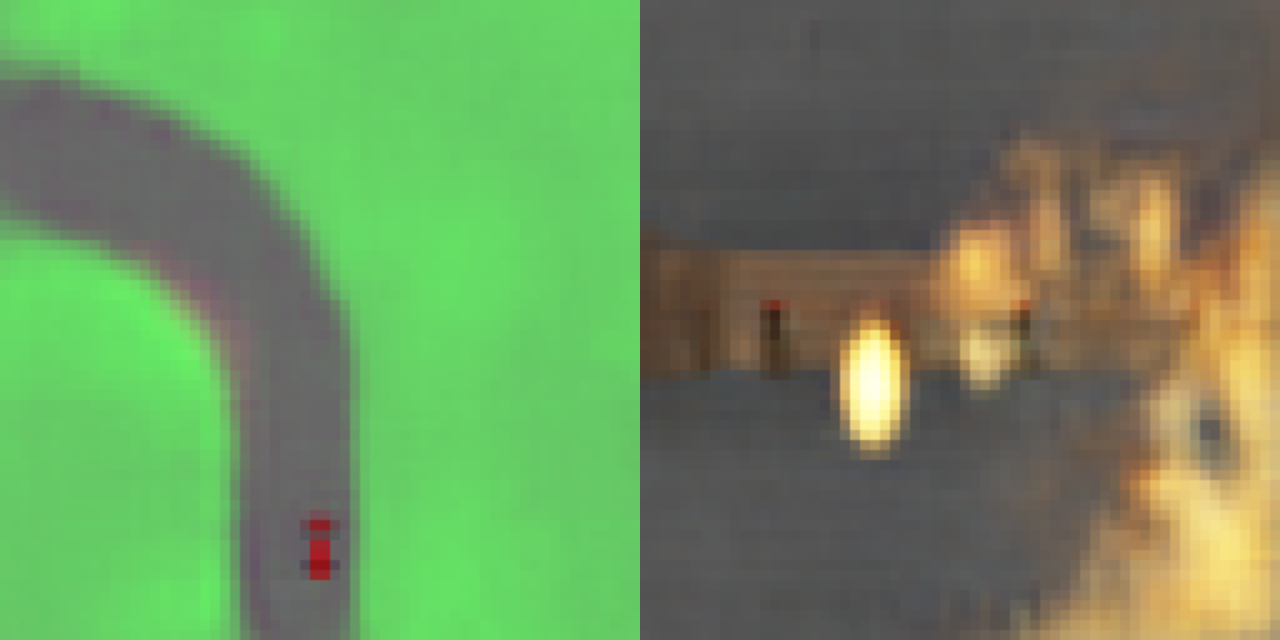
\includegraphics[width=1.0\columnwidth]{assets/world_models_card_both.png}}
\vskip -0.05in
\caption{本文为 OpenAI Gym 环境构建概率生成模型。基于 RNN 的世界模型使用真实游戏环境中记录的观测数据训练。训练完成后，这些世界模型可以模拟完整环境，并用于训练智能体。}
\end{center}
\vskip -0.25in
\end{figure}
%A simple example is training an agent to play Flappy Bird~\cite{flappy_bird} from observing only pixel inputs. If the agent had already learned a compressed, low-dimensional representation of each image frame it sees, and also a predictive model of what the frames will look like in the future, then it would have almost all of the information needed to solve this task \cite{keras_flappybird}。
%\begin{figure}[ht]
%\vskip -0.0in
%\begin{center}
%\centerline{\includegraphics[width=1.0\columnwidth]{assets/flappy_bird_multi.jpeg}}
%\caption{Flappy Bird Clone \cite{flappy_bird_ne}}
%\label{flappy_bird_clone_figure}
%\end{center}
%\vskip -0.3in
%\end{figure}
大型 RNN 容量较高，能够学习空间和时间表示。然而，文献中的许多\textit{无模型} RL 方法往往只使用参数较少的小型神经网络。RL 算法常受信用分配问题限制，传统方法很难直接学习包含数百万权重的大模型。因此实践中通常使用较小网络，因为它们能在训练过程中更快迭代到可用策略。

理想情况下，我们希望能够高效训练大型 RNN 智能体。反向传播算法\cite{Linnainmaa:1970,Kelley:1960,werbos1982sensitivity} 可以高效训练大型神经网络。本文关注一种面向 RL 任务的分解方式：把智能体拆分为大型世界模型和小型控制器模型\footnote{典型无模型 RL 模型大约有 $10^3$ 到 $10^6$ 个参数。本文训练约 $10^7$ 参数量级的模型；与 $10^8$ 甚至 $10^9$ 参数的先进深度学习模型相比，这仍然不算大。原则上，本文流程也可以利用更大的网络。}。我们先以无监督方式训练大型神经网络来学习智能体所处世界的模型，再训练较小控制器利用该世界模型完成任务。小控制器将训练算法的信用分配问题限制在较小搜索空间内，同时让世界模型承担主要表示学习工作。实验表明，在世界模型视角下训练智能体，可以学到很紧凑的任务策略。

尽管已有大量研究讨论\textit{基于模型}的强化学习，本文并不试图综述该领域现状\cite{rl_survey,s03_overview}。我们的目标是从 1990--2015 年一系列关于 RNN 世界模型与控制器组合的工作中提炼若干关键概念\cite{s05_making_the_world_differentiable,s05a_cm,s05b_rl,s05c_boredom,learning_to_think}。我们也会讨论文献中其他相关工作，它们同样关注学习世界模型，并训练智能体使用该模型。

本文提出一个简化框架，用于实验性展示上述工作的若干核心思想，并进一步讨论如何将这些思想有效应用到不同 RL 环境中。在描述方法和实验时，我们沿用 \textit{On Learning to Think: Algorithmic Information Theory for Novel Combinations of RL Controllers and RNN World Models}\cite{learning_to_think} 中相近的术语与记号。
\vskip -0.15in
\section{智能体模型}
\vskip -0.05in
我们提出一个受人类认知系统启发的简单模型。在该模型中，智能体包含一个视觉感知组件，用于把看到的内容压缩成小型表示代码；一个记忆组件，用于根据历史信息预测未来代码；以及一个决策组件，只根据视觉和记忆组件产生的表示来决定采取何种动作。

\begin{figure}[ht]
\vskip -0.05in
\begin{center}
\centerline{\includegraphics[width=1.0\columnwidth]{svg/world_model_overview.pdf}}
\vskip -0.0in
\caption{智能体由三个紧密协作的组件构成：\textbf{Vision (V)}、\textbf{Memory (M)} 和 \textbf{Controller (C)}。}
\label{overview_diagram_figure}
\end{center}
\vskip -0.3in
\end{figure}

\subsection{VAE(V)模型}
\vskip -0.05in
环境在每个时间步向智能体提供高维输入观测。该输入通常是视频序列中的一帧 2D 图像。V 模型的作用是为每个观测图像帧学习抽象且压缩的表示。

\begin{figure}[ht]
\vskip -0.0in
\begin{center}
\centerline{\includegraphics[width=1.0\columnwidth]{svg/vae.pdf}}
\caption{变分自动编码器(VAE)的流程图。}
\label{vae_figure}
\end{center}
\vskip -0.3in
\end{figure}

这里使用一个简单的变分自动编码器\cite{vae,vae_dm} 作为 V 模型，将每个图像帧压缩为一个小型\textit{潜在向量} $z$。

\subsection{MDN-RNN(M)模型}

V 模型负责压缩智能体在每个时间步看到的内容；我们还希望压缩随时间展开的动态变化。为此，M 模型负责预测未来，具体来说，它预测 V 模型将产生的未来潜在向量 $z$。由于许多复杂环境本身具有随机性，我们训练 RNN 输出概率密度函数 $p(z)$，而不是对 $z$ 给出单点确定性预测。

\begin{figure}[ht]
\vskip -0.15in
\begin{center}
\centerline{\includegraphics[width=0.85\columnwidth]{svg/mdn_rnn_new.pdf}}
\vskip -0.10in
\caption{带混合密度网络输出层的 RNN。MDN 输出高斯混合分布的参数，用于采样下一个潜在向量 $z$ 的预测值。}
\label{mdn_rnn_new_figure}
\end{center}
\vskip -0.25in
\end{figure}

在本文方法中，我们用高斯混合分布近似 $p(z)$，并训练 RNN 在给定当前和历史信息的条件下，输出下一个潜在向量 $z_{t+1}$ 的概率分布。

更具体地说，RNN 建模 $P(z_{t+1} \; | \; a_t, z_t, h_t)$，其中 $a_t$ 是时间 $t$ 采取的动作，$h_t$ 是 RNN 在时间 $t$ 的\textit{隐藏状态}。采样时，我们可以像 \cite{sketchrnn} 那样调节\textit{温度}参数 $\tau$ 来控制模型不确定性；后文会看到，调节 $\tau$ 对训练控制器很有用。

\begin{figure}[ht]
\vskip -0.0in
\begin{center}
\centerline{\includegraphics[width=1.0\columnwidth]{svg/sketchrnn.pdf}}
\caption{SketchRNN\cite{sketchrnn} 是 MDN-RNN 的一个例子，用于预测草图绘制中的下一笔。本文使用类似模型来预测下一个潜在向量 $z_t$。}
\label{sketchrnn_figure}
\end{center}
\vskip -0.2in
\end{figure}

这种方法被称为混合密度网络\cite{bishop} 与 RNN(MDN-RNN)相结合\cite{graves_rnn,mdnrnn_tutorial}，过去用于生成笔迹等序列生成问题\cite{graves_rnn} 和草图\cite{sketchrnn}。

\subsection{控制器(C)模型}

控制器(C)模型负责决定动作序列，使智能体在环境 rollout 期间的期望累积奖励最大化。在实验中，我们有意让 C 尽可能简单、尽可能小，并将其与 V 和 M 分开训练，使主要建模负担落在世界模型(V 和 M)上。

C 是一个简单的单层线性模型，在每个时间步把 $z_t$ 和 $h_t$ 直接映射为动作 $a_t$：
\vskip -0.1in
\begin{equation}
\label{controller_equation}
a_t = W_c \; [z_t \; h_t]\; + b_c
\end{equation}
\vskip -0.00in
在该线性模型中，$W_c$ 和 $b_c$ 分别是权重矩阵和偏置向量，将拼接后的输入向量 $[z_t \; h_t]$ 映射到输出动作向量 $a_t$。

\subsection{组合 V、M 和 C}

下图说明 V、M、C 与环境之间的交互：

\begin{figure}[ht]
\vskip -0.0in
\begin{center}
\centerline{\includegraphics[width=0.70\columnwidth]{svg/world_model_schematic.pdf}}
\caption{智能体模型流程图。原始观测首先在每个时间步 $t$ 由 V 处理，产生 $z_t$。C 的输入是潜在向量 $z_t$ 与 M 的隐藏状态 $h_t$ 的拼接；C 随后输出动作向量 $a_t$，该动作会影响环境。M 接收当前 $z_t$ 和动作 $a_t$，更新自身隐藏状态并产生将在时间 $t+1$ 使用的 $h_{t+1}$。}
\label{world_model_schematic_figure}
\end{center}
\vskip -0.3in
\end{figure}

下面给出在 OpenAI Gym~\cite{openai_gym} 环境中使用该智能体模型的伪代码：
\begin{verbatim}
def rollout(controller):
 ''' env, rnn, vae are '''
 ''' global variables '''
 obs = env.reset()
 h = rnn.initial_state()
 done = False
 cumulative_reward = 0
 while not done:
 z = vae.encode(obs)
 a = controller.action([z, h])
 obs, reward, done = env.step(a)
 cumulative_reward += reward
 h = rnn.forward([a, z, h])
 return cumulative_reward
\end{verbatim}

给定控制器 C 后，运行该函数会返回一次 rollout 的累积奖励。

C 的极简设计也有实践好处。深度学习的发展使我们能够高效训练大型复杂模型，但前提是可以定义合适且可微的损失函数。V 和 M 被设计为可用现代 GPU 加速器通过反向传播高效训练，因此我们把大部分参数放在 V 与 M 中。相比之下，C 是一个线性模型，参数量很小。这一选择使我们能够探索更非常规的 C 训练方式，例如在信用分配困难的 RL 任务中使用进化策略(ES)~\cite{Rechenberg1973,Schwefel1977}。

为优化 C 的参数，我们选择协方差矩阵自适应进化策略(CMA-ES)~\cite{cmaes,cmaes_original}。该算法已知可以较好地处理多达数千维参数的搜索空间。我们在一台具有多个 CPU 核心的机器上演化 C 的参数，并并行运行多个环境 rollout。

关于实验中使用的模型、训练流程和环境设置，更多细节见附录。

\section{汽车赛跑实验}

本节说明如何训练前述智能体模型来解决赛车任务。据我们所知，这是第一个达到该任务“解决”分数要求的已知智能体。\footnote{我们认为该任务值得研究，因为在 \texttt{CarRacing-v0} 中，让智能体围绕随机生成的赛道行驶并取得一般分数并不困难；但要达到 \textit{solving} 定义的标准，智能体只能出现极少量驾驶失误。}

\subsection{世界模型作为特征提取器}

预测性世界模型可以帮助我们学习有用的空间和时间表示。将这些表示作为控制器输入后，可以训练一个紧凑的最小控制器来完成连续控制任务。例如，在 \texttt{CarRacing-v0}~\cite{carracing_v0} 这个自上而下的赛车环境中，智能体需要直接从像素输入学习驾驶。

\begin{figure}[ht]
\vskip -0.0in
\begin{center}
\centerline{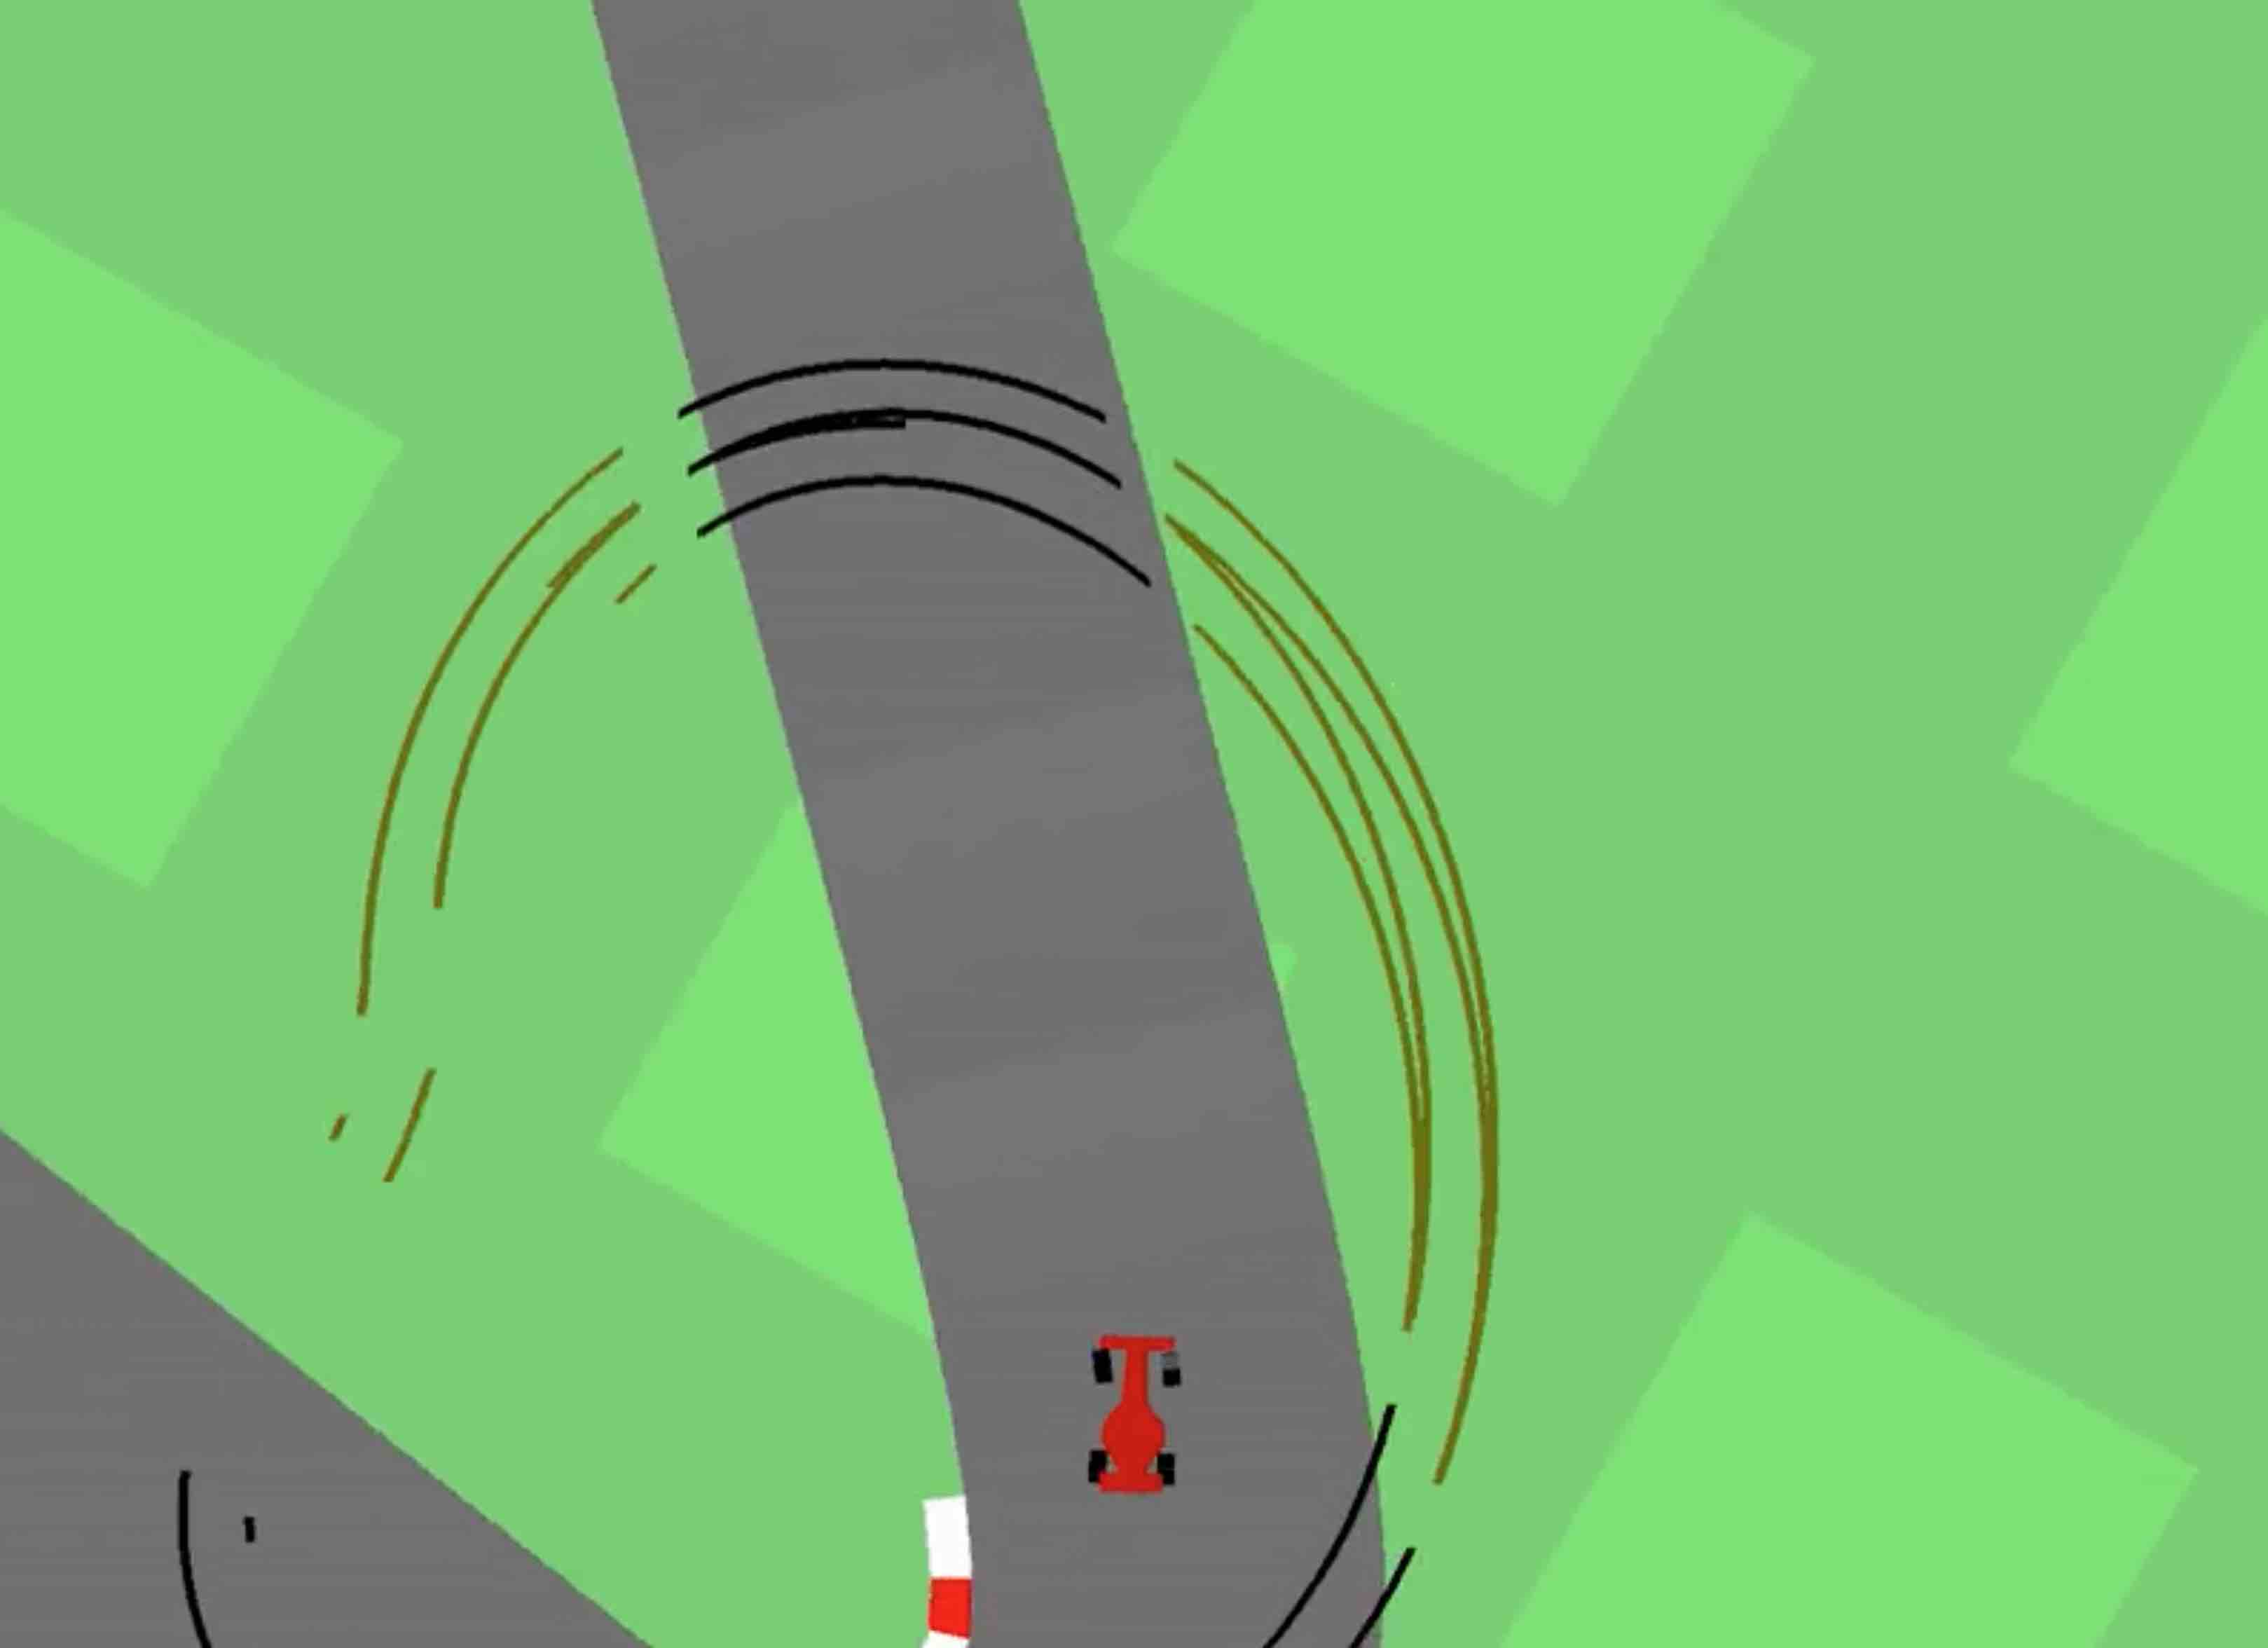
\includegraphics[width=1.0\columnwidth]{mp4/carracing_mistake_short.jpeg}}
\caption{智能体正在学习在 \texttt{CarRacing-v0} 中驾驶。}
\end{center}
\vskip -0.3in
\end{figure}

在该环境中，每次试验都会随机生成赛道。智能体需要在尽可能短的时间内经过尽可能多的赛道格子，并据此获得奖励。智能体控制三个连续动作：左/右转向、油门和刹车。

为训练 V 模型，我们首先收集 10,000 次随机环境 rollout 的数据。具体做法是让智能体随机探索环境，并记录随机动作 $a_t$ 及对应观测。我们用该数据集训练 V，使其学习每个观测帧的潜在空间表示。VAE 被训练为将每帧编码成低维潜在向量 $z$，并最小化原始帧与解码器从 $z$ 重建出的图像之间的差异。

随后，我们可以用训练好的 V 模型把时间 $t$ 的每一帧预处理为输入 $z_t$。利用这些预处理后的数据以及记录下来的随机动作 $a_t$，MDN-RNN 可以被训练来把 $P(z_{t+1} \; | \; a_t, z_t, h_t)$ 建模为高斯混合分布。\footnote{原则上，两个模型可以端到端联合训练；但我们发现分别训练更实用，结果也足够好。每个模型的训练时间不到一小时，我们也能在不大量调参的情况下分别训练 VAE 和 MDN-RNN。}

在该实验中，世界模型(V 和 M)完全不知道环境中的真实奖励信号；它的任务只是压缩并预测观测到的图像帧序列。只有控制器(C)能够访问环境奖励。由于线性控制器只有 867 个参数，CMA-ES 等进化算法很适合这一优化任务。

我们可以使用 VAE 重建每个框架$z_t$下图显示通过截图训练的 VAE 模型。\texttt{CarRacing-v0}。

\begin{figure}[ht]
\vskip -0.0in
\begin{center}
\centerline{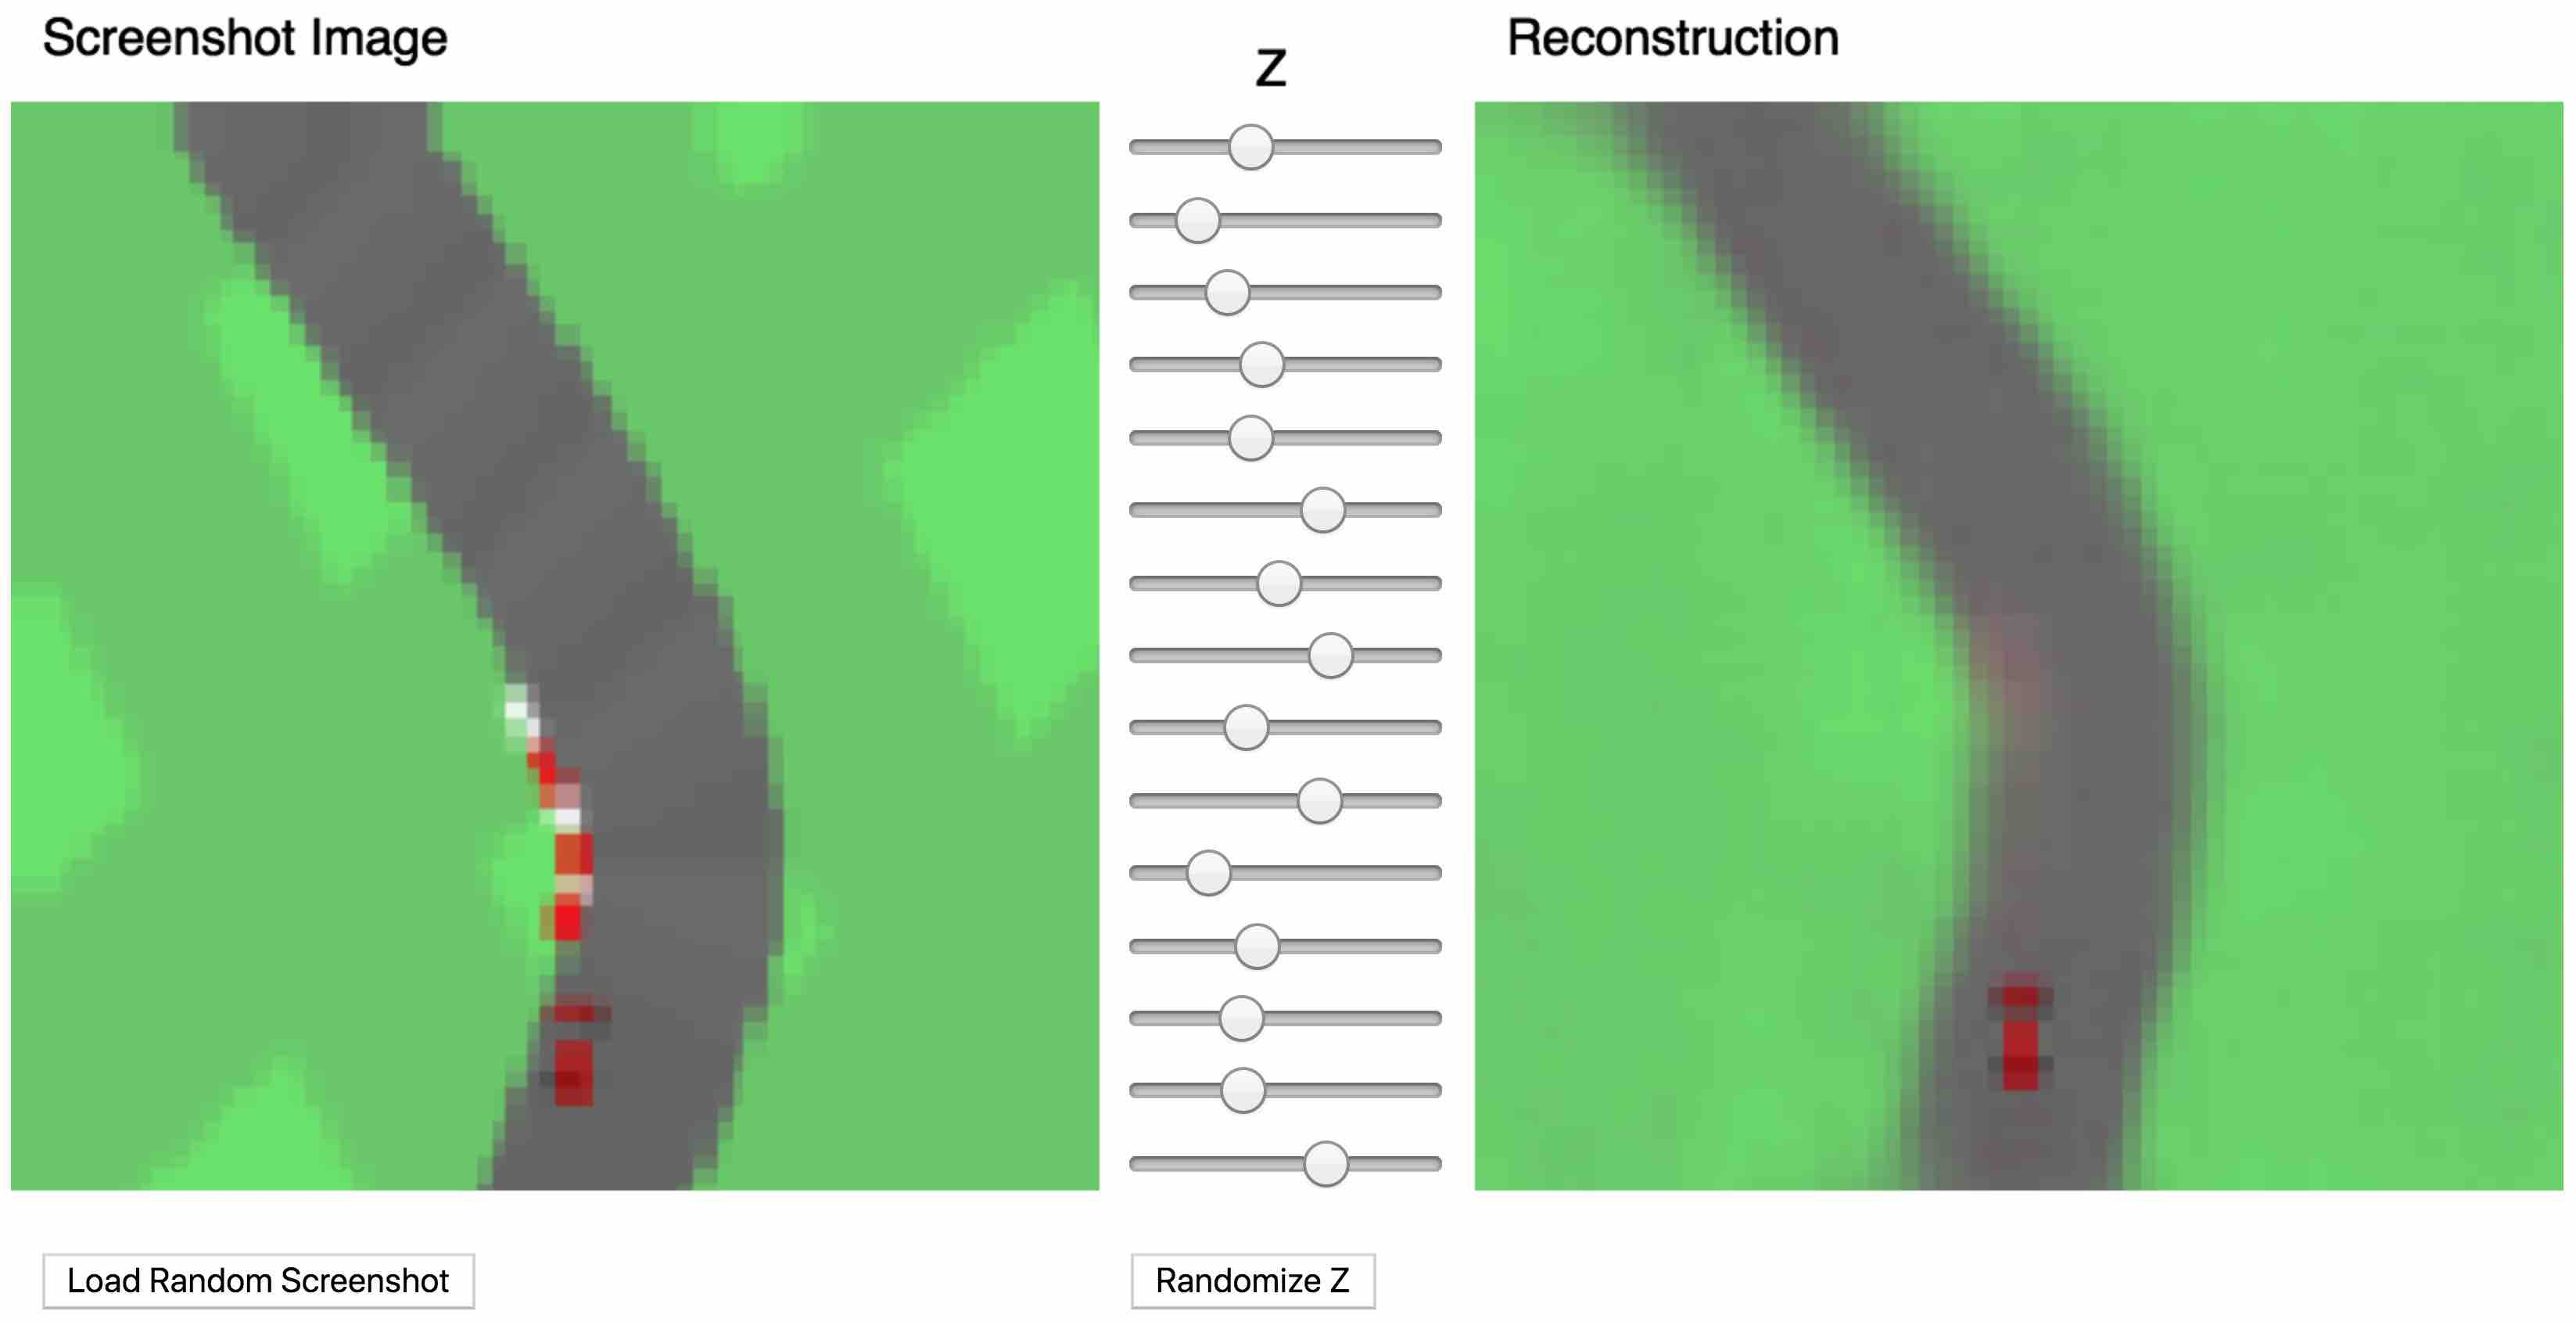
\includegraphics[width=1.0\columnwidth]{demo/demo_carracing_vae.jpeg}}
\caption{尽管有损压缩会丢失部分细节，潜在向量 $z$ 仍能捕捉每个图像帧的关键信息。}
\end{center}
\vskip -0.3in
\end{figure}

在本文在线版本中，读者可以加载随机选择的截图，将其编码为小型潜在向量 $z$ 并重建原始截图；也可以用滑块调整该截图的 $z$ 向量，观察重建结果如何变化，或随机采样 $z$ 来探索可能截图的空间。

\subsection{程序}

汽车赛跑实验流程如下：

\begin{enumerate}
 \item 从随机策略收集 10,000 次 rollout。
 \item 训练 VAE(V)，将图像帧编码为 $z \in \mathcal{R}^{32}$。
 \item 训练 MDN-RNN(M)，建模 $P(z_{t+1} \; | \; a_t, z_t, h_t)$。
 \item 定义控制器(C)：$a_t = W_c \; [z_t \; h_t]\; + \; b_c$。
 \item 使用 CMA-ES 求解 $W_c$ 和 $b_c$，最大化期望累积奖励。
\end{enumerate}

\begin{table}[ht]
\label{car_racing_param_count_table}
\vskip -0.0in
\begin{center}
\begin{small}
\begin{sc}
\begin{tabular}{lc}
\toprule
模型&参数量\\
\midrule
VAE& 4,348,547 \\
MDN-RNN& 422,368 \\
Controller& 867 \\
\bottomrule
\end{tabular}
\end{sc}
\end{small}
\end{center}
\vskip -0.0in
\end{table}

\subsection{实验结果}
\medskip
\textit{V 模型}

如果观测表示足够好，训练一个驾驶智能体并不困难。已有项目\cite{browser_car,mar_io_kart,keras_car} 表明，只要提供一组人工设计的观测特征，例如 LIDAR 信息、角度、位置和速度，就很容易训练一个小型前馈网络接收这些输入并输出可用的导航策略。基于这一点，我们首先通过禁用 M 来测试智能体，使控制器只能访问 V 而不能访问记忆状态，此时控制器定义为 $a_t = W_c \; z_t \;+ \; b_c$。

\begin{figure}[ht]
\vskip -0.0in
\begin{center}
\centerline{
\includegraphics[width=1.0\columnwidth]{mp4/carracing_v_only.jpeg}}
\caption{当控制器只能看到 $z_t$ 而无法访问 $h_t$ 时，驾驶行为较弱且不稳定。}
\end{center}
\vskip -0.3in
\end{figure}

虽然该智能体仍能沿赛道行驶，但我们观察到它会左右摆动，并在较急的弯道处偏离赛道。这个受限智能体在 100 次随机试验中的平均得分为 $632\pm251$，与 OpenAI Gym 排行榜上的其他智能体~\cite{carracing_v0} 以及 A3C 等传统深度 RL 方法\cite{carracing_cs221,carracing_cs234} 大致相当。在 C 策略网络中加入一个隐藏层可以把结果提升到 $788\pm141$，但仍不足以解决该环境。

\medskip

\textit{完整世界模型。}

相比只使用 $z_t$，M 被训练来完成一件事，并且尽可能做好：预测 $z_{t+1}$。由于 M 对 $z_{t+1}$ 的预测来自时间 $t$ 的 RNN 隐藏状态 $h_t$，这个向量自然可以作为一组学习到的特征提供给智能体。把 $z_t$ 与 $h_t$ 结合起来，就能让控制器 C 同时获得当前观测和对未来的预期表示。

\begin{figure}[ht]
\vskip -0.0in
\begin{center}
\centerline{
\includegraphics[width=1.0\columnwidth]{mp4/carracing_v_and_m.jpeg}}
\caption{当控制器同时访问 $z_t$ 和 $h_t$ 时，驾驶行为更加稳定。}
\end{center}
\vskip -0.4in
\end{figure}

可以看到，让智能体同时访问 $z_t$ 和 $h_t$ 后，驾驶能力显著提升，行驶更稳定，也更能处理急弯。此外，在赛车过程中作出快速反应式驾驶决策时，智能体不需要显式规划未来并展开多个假设场景。由于 $h_t$ 包含关于未来概率分布的信息，智能体可以直接查询 RNN 表示来指导动作决策。类似经验丰富的一级方程式车手或前文提到的棒球击球手，智能体能够基于内部预测快速判断何时、向何处行动。

\begin{table}[ht]
\label{car_racing_table}
\vskip -0.0in
\begin{center}
\begin{small}
\begin{sc}
\begin{tabular}{ll}
\toprule
方法&积分\\
\midrule
DQN~\cite{dqn_racecar} & 343 $\pm$ 18 \\
A3C(持续)~\cite{carracing_cs234} & 591 $\pm$ 45 \\
A3C(分别)~\cite{carracing_cs221} & 652 $\pm$ 10 \\
亿万富翁& 838 $\pm$ 11 \\
V型号& 632 $\pm$ 251 \\
V 型号带有隐藏层& 788 $\pm$ 141 \\
\textbf{满World Model} & \textbf{906 $\pm$ 21} \\
\bottomrule
\end{tabular}
\end{sc}
\end{small}
\end{center}
\vskip -0.2in
\caption{\texttt{CarRacing-v0} 使用各种方法取得的分数。}
\vskip -0.1in
\end{table}

我们的智能体在 100 次随机试验中达到 $906\pm21$ 分，已经有效解决该任务，并取得当时的最优结果。使用深度 RL 的方法\cite{carracing_cs221,carracing_cs234} 平均分通常在 591--652 之间，排行榜上报告的最佳方案为 $838\pm11$（100 次随机试验）。传统深度 RL 方法往往需要逐帧预处理，例如边缘检测\cite{carracing_cs234}，并叠加最近若干帧作为输入\cite{carracing_cs221,carracing_cs234}。相比之下，本文的世界模型直接从原始 RGB 像素流中学习时空表示。据我们所知，这是首个公开报告的、能够解决该任务的方法。

\subsection{汽车赛车梦}

由于世界模型能够模拟未来，我们也可以让它生成假想的赛车场景。给定当前状态后，M 会产生关于 $z_{t+1}$ 的概率分布；从中\textit{采样}一个 $z_{t+1}$，就可以把训练好的 C 放回由 M 生成的幻觉环境中运行。下图来自本文在线版本中的交互式演示。

\begin{figure}[ht]
\vskip -0.0in
\begin{center}
\centerline{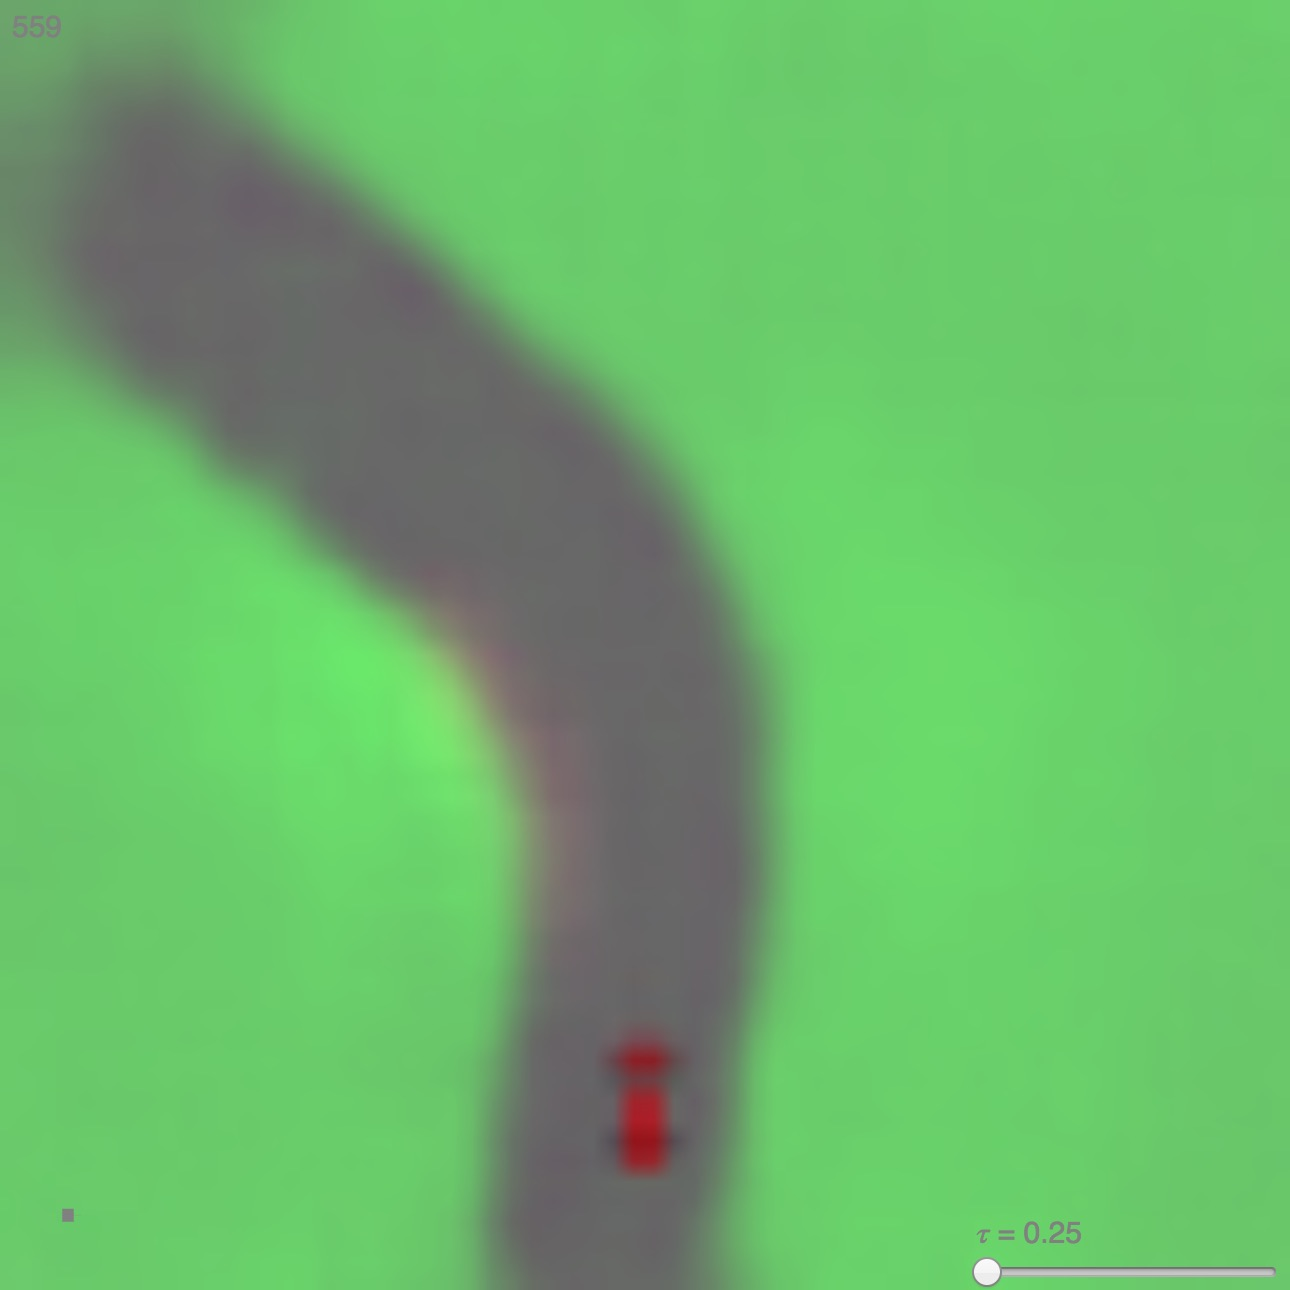
\includegraphics[width=1.0\columnwidth]{demo/demo_carracing_rnn.jpeg}}
\caption{智能体驶入自己的梦境世界。这里将训练好的策略应用到由 MDN-RNN 生成的虚拟环境中，并用 VAE 解码器渲染画面。在演示中，读者可以覆盖智能体动作，也可以调节 $\tau$ 来控制 M 生成环境的不确定性。}
\end{center}
\vskip -0.4in
\end{figure}

\section{VizDoom 实验}

\subsection{在梦中学习}

前面看到，在真实环境中学到的策略似乎也能在梦境环境中发挥作用。这自然引出一个问题：能否让智能体完全在自己的梦中学习，再把学到的策略迁移回真实环境？

如果世界模型对当前任务足够准确、足够完整，那么它应当可以替代真实环境。毕竟，智能体并不直接观察“现实”，它看到的是世界模型允许它看到的内容。在这个实验中，我们让世界模型模仿 VizDoom\cite{vizdoom} 环境，并在该模型生成的幻觉中训练智能体。

\begin{figure}[ht]
\vskip -0.0in
\begin{center}
\centerline{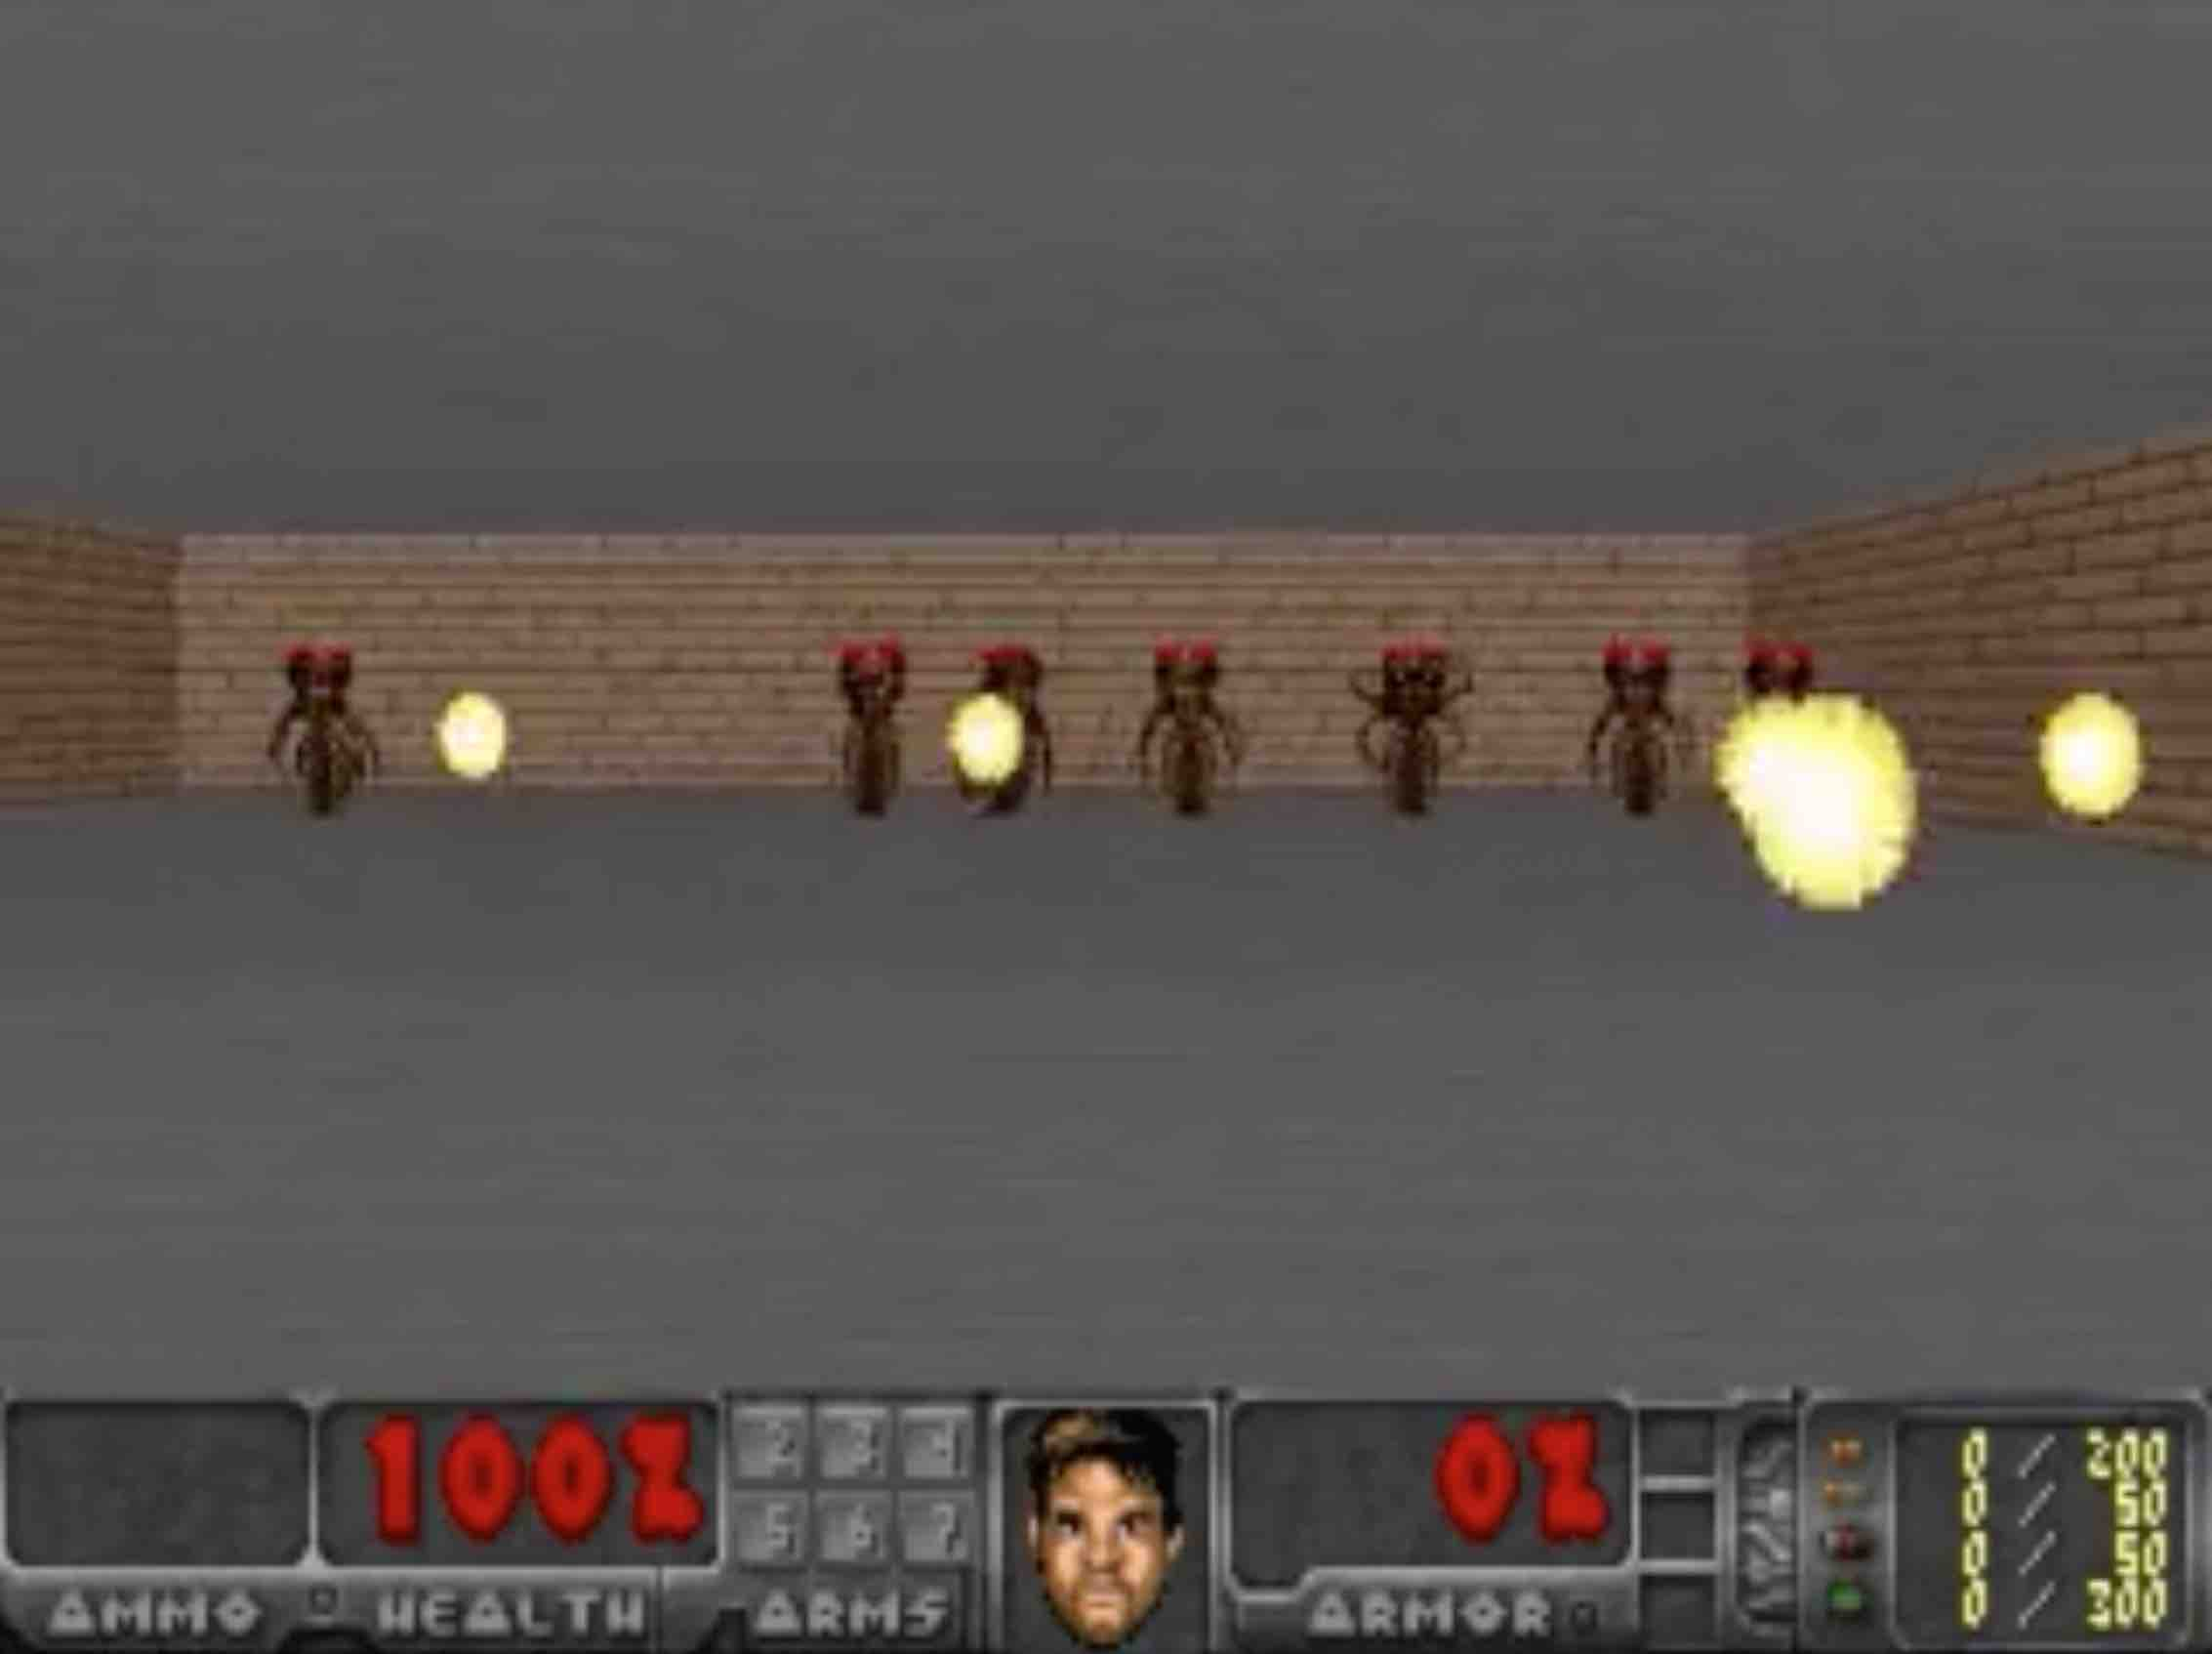
\includegraphics[width=1.0\columnwidth]{mp4/doom_lazy_small.jpeg}}
\caption{最终智能体解决 \textit{VizDoom: Take Cover}。}
\end{center}
\vskip -0.4in
\end{figure}

智能体必须学会躲避房间另一侧怪物发射的火球。在该环境中没有显式奖励，因此为了模拟自然选择，我们把累积奖励定义为智能体在一次 rollout 中存活的时间步数。每次环境 rollout 最多持续 2100 个时间步（约 60 秒）；若连续 100 次 rollout 的平均存活时间超过 750 个时间步（约 20 秒），任务即视为解决~\cite{takecover}。

\subsection{程序}

VizDoom 实验的设置与 CarRacing 基本相同，但有几处关键区别。在 CarRacing 中，M 只被训练来建模下一个 $z_t$。由于这里的目标是构建一个可用于训练智能体的完整世界模型，M 除了预测下一帧 $z_t$ 外，还要预测智能体是否会在下一帧死亡，即二值事件 $done_t$，简写为 $d_t$。

由于 M 模型除了下一观测外还能预测 $done$ 状态，我们已经具备构建完整 RL 环境所需的要素。我们把 M 包装成一个 \texttt{gym.Env} 接口，就像它是真实 Gym 环境一样，然后在这个\textit{虚拟}环境中训练智能体，而不是直接使用真实环境。

在该模拟中，幻觉过程不再需要 V 模型去编码真实像素帧，因此智能体完全在潜在空间环境中训练。后文会看到，这带来若干实际好处。

虚拟环境与真实环境具有相同接口。因此，智能体在虚拟环境中学到满意策略后，可以直接把该策略部署回真实环境，检验迁移效果。

总结 \textit{Take Cover} 实验，流程如下：

\begin{enumerate}
 \item 从随机策略收集 10,000 次 rollout。
 \item 训练 VAE(V)，将每帧编码为潜在向量 $z \in \mathcal{R}^{64}$，并用 V 将步骤(1)收集的图像转换为潜在空间表示。
 \item 训练 MDN-RNN(M)，建模\\ $P(z_{t+1}, d_{t+1} \; | \; a_t, z_t, h_t)$。
 \item 定义控制器(C)：$a_t = W_c \; [z_t \; h_t]$。
 \item 使用 CMA-ES 求解 $W_c$，在虚拟环境中最大化期望存活时间。
 \item 将步骤(5)学到的策略应用到真实环境。
\end{enumerate}

\begin{table}[ht]
\label{doom_cover_table}
\vskip -0.0in
\begin{center}
\begin{small}
\begin{sc}
\begin{tabular}{lc}
\toprule
模型&参数量\\
\midrule
VAE& 4,446,915 \\
MDN-RNN& 1,678,785 \\
Controller& 1,088 \\
\bottomrule
\end{tabular}
\end{sc}
\end{small}
\end{center}
\vskip -0.0in
\end{table}

\subsection{梦中的训练}

经过训练后，控制器学会在梦境环境中移动，并躲避由 M 生成的怪物发射的致命火球。智能体在虚拟环境中的\textit{得分}约为 900 个时间步。

\begin{figure}[ht]
\vskip -0.0in
\begin{center}
\centerline{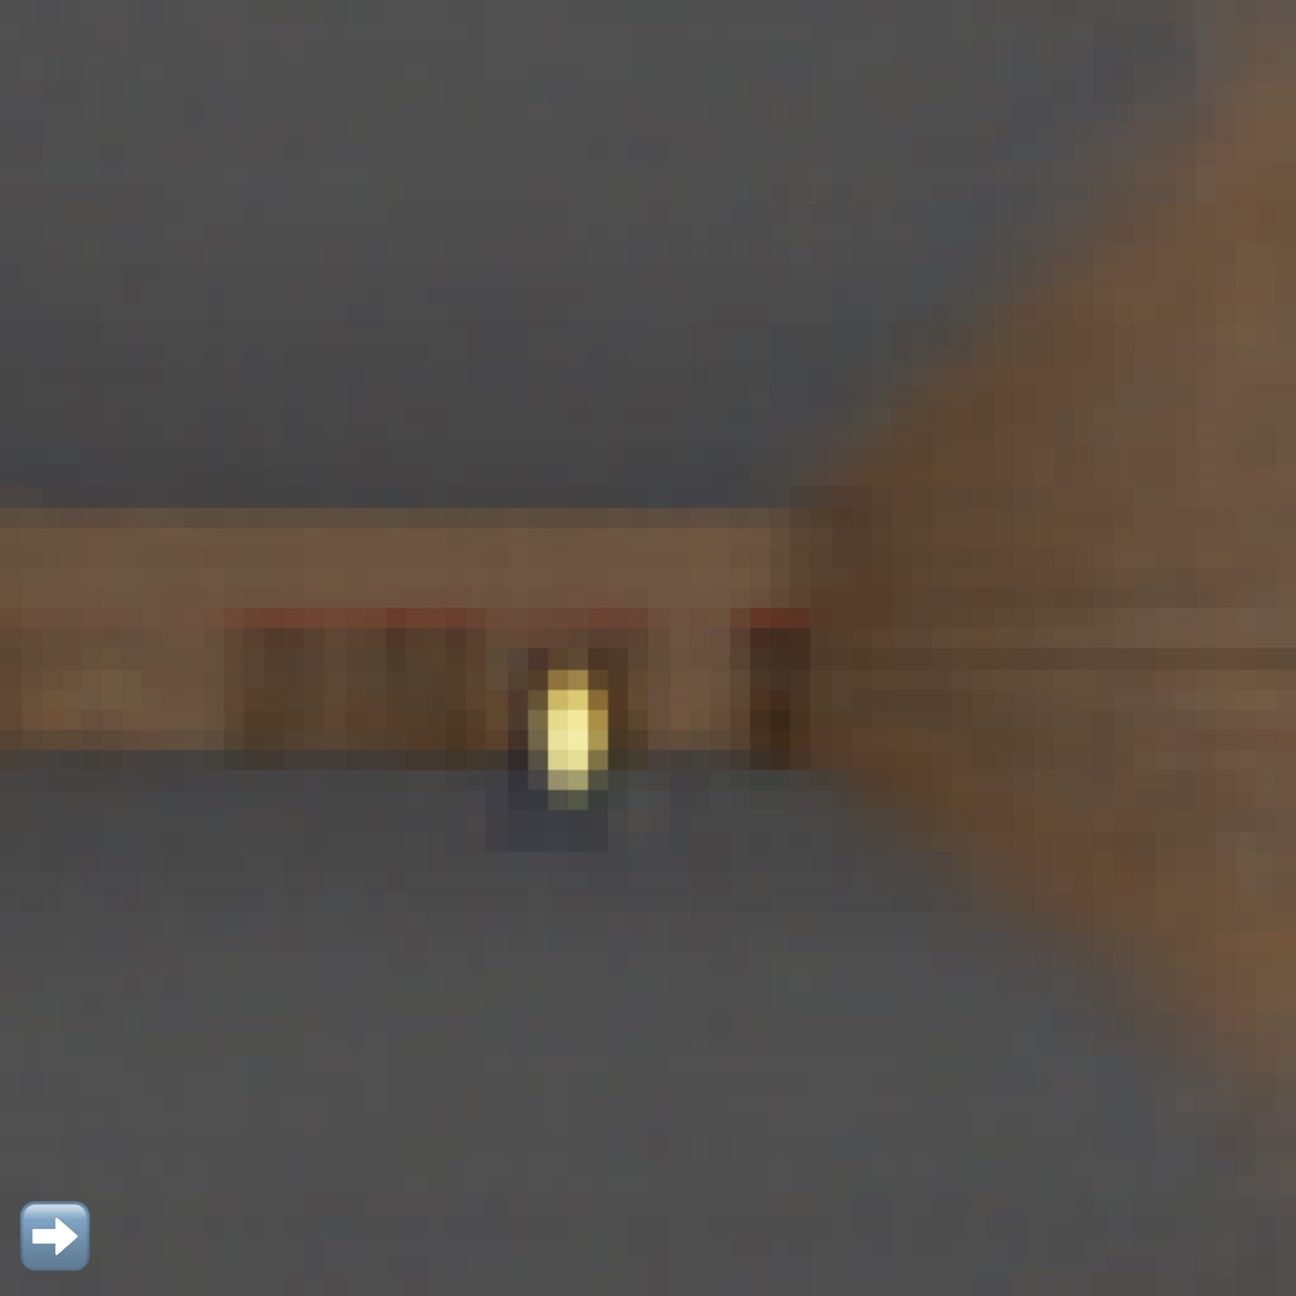
\includegraphics[width=1.0\columnwidth]{demo/demo_doom_rnn.jpeg}}
\vskip -0.1in
\caption{智能体发现了躲避幻觉火球的策略。在本文在线版本中，读者可以与该演示环境交互。}
\end{center}
\vskip -0.4in
\end{figure}

这里，基于 RNN 的世界模型被训练来模仿由人类程序员设计的完整游戏环境。它只从随机 episode 收集的原始图像数据中学习，却能够模拟游戏的若干基本方面，包括游戏逻辑、敌人行为、物理效果以及 3D 图形渲染。

例如，如果智能体选择向左移动，M 模型会学会把智能体移向左侧，并相应调整其内部游戏状态表示。如果智能体试图朝任一方向移动过远，模型也会学会阻止其穿过关卡两侧墙壁。有时，M 需要同时跟踪由多个怪物发射的多枚火球，并让它们沿各自方向一致移动；它还必须检测智能体是否被某个火球击中。

不过，与真实游戏环境不同，我们可以在虚拟环境中加入额外不确定性，使梦境环境更具挑战。具体做法是在采样 $z_{t+1}$ 时增大温度参数 $\tau$。不确定性增加后，梦境环境会比真实环境更困难；火球的移动路径可能比真实游戏中更随机、更难预测。有时智能体甚至会因为单纯运气不好而死亡。

我们发现，在较高温度设置下表现良好的智能体，通常在正常环境中也表现更好。事实上，提高 $\tau$ 有助于防止控制器利用世界模型的缺陷；这一点稍后会进一步讨论。

\subsection{向真实环境迁移策略}

\begin{figure}[ht]
\vskip -0.0in
\begin{center}
\centerline{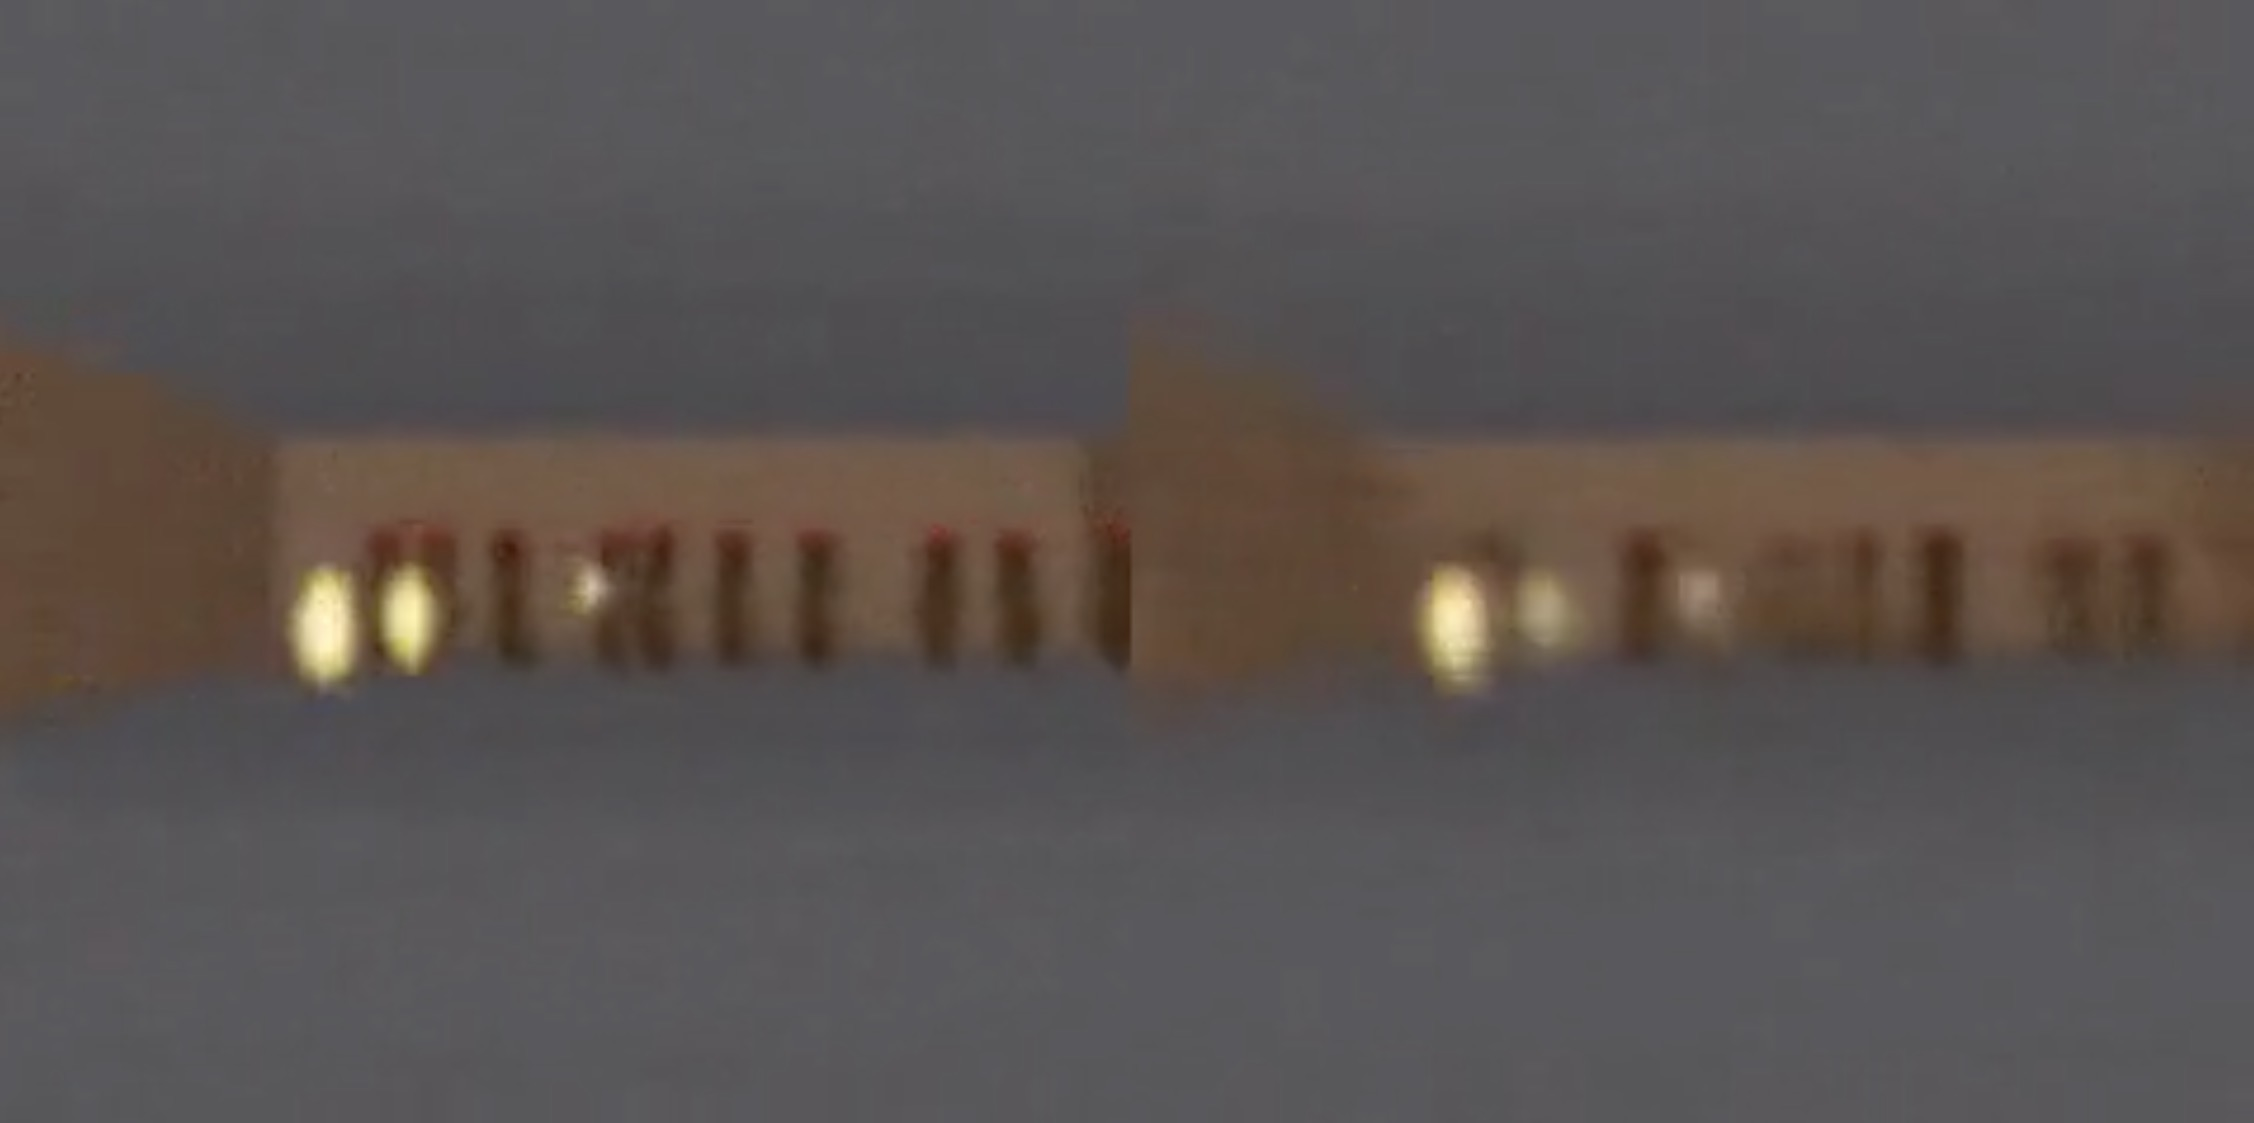
\includegraphics[width=1.0\columnwidth]{mp4/doom_real_vae.jpeg}}
\vskip -0.1in
\caption{将在梦境 RNN 环境中学到的策略部署回真实 VizDoom 环境。}
\end{center}
\vskip -0.2in
\end{figure}

我们将虚拟环境中训练出的智能体带回原始 VizDoom 场景中测试。在 100 次连续随机试验中，它的得分约为 1100 个时间步，远高于任务要求的 750 个时间步，也明显高于其在更困难虚拟环境中的得分。

\begin{figure}[ht]
\vskip -0.0in
\begin{center}
\centerline{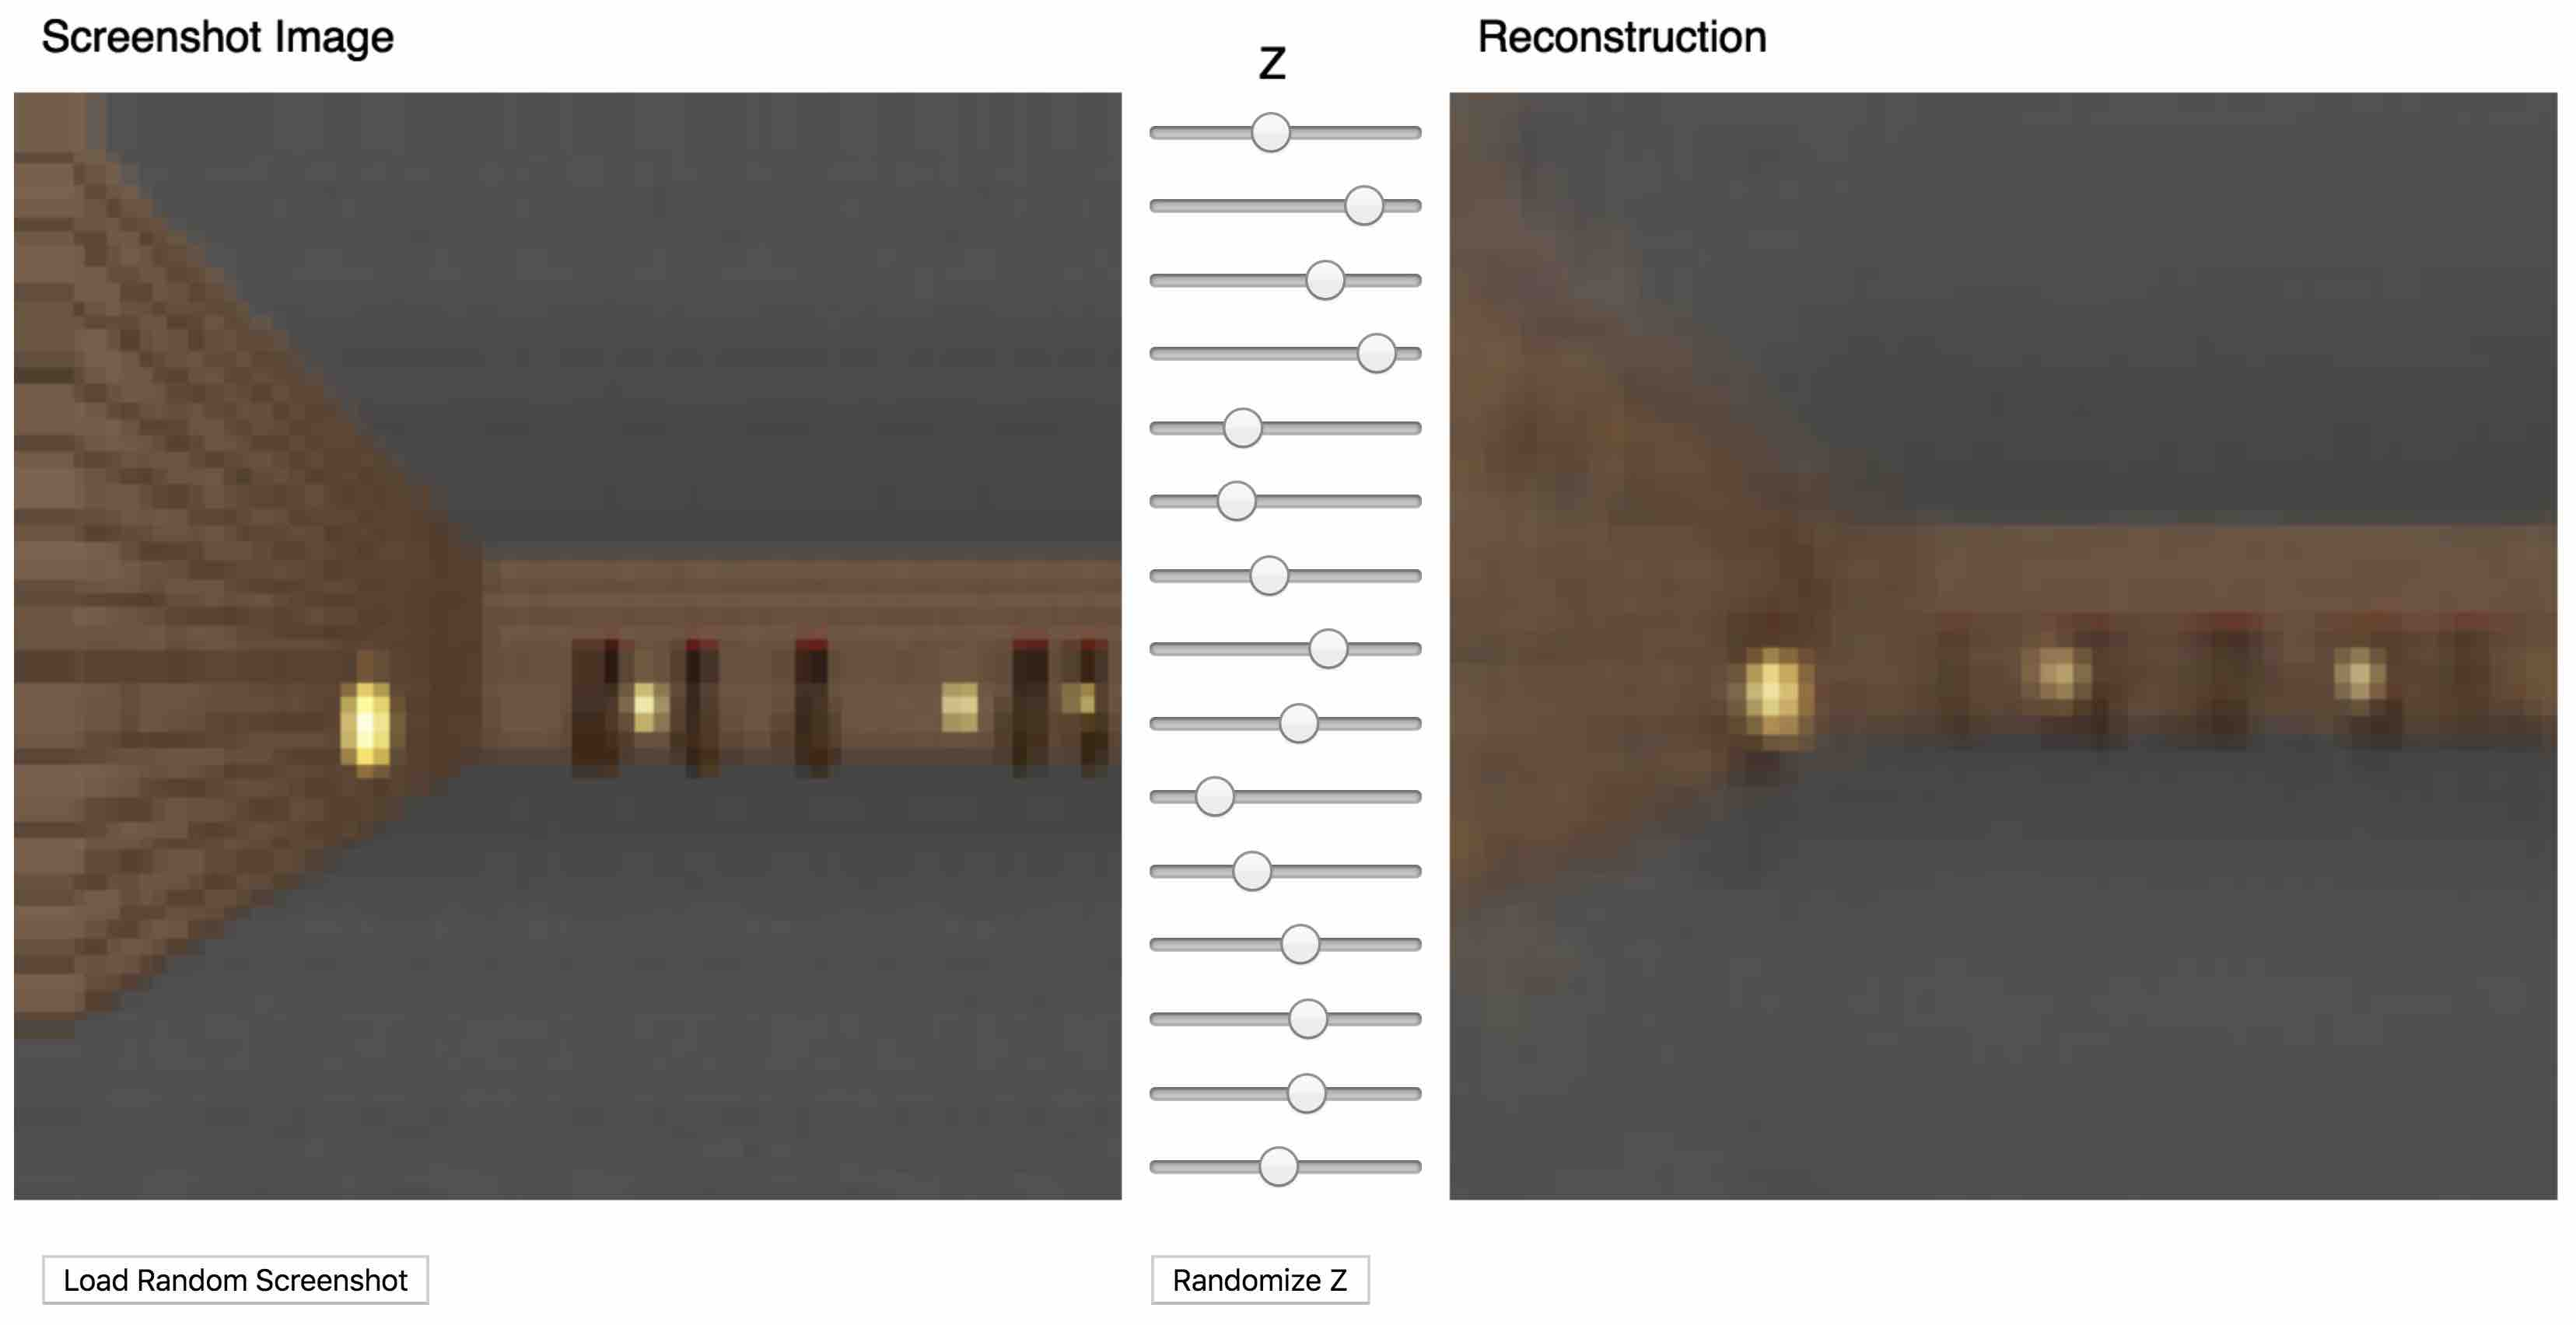
\includegraphics[width=1.0\columnwidth]{demo/demo_doom_vae.jpeg}}
\caption{在线文章中的 Doom 交互式 VAE。}
\vskip -0.15in
\end{center}
\vskip -0.25in
\end{figure}

可以看到，尽管 V 模型无法准确捕捉每帧中的所有细节，例如怪物数量并不总是正确，智能体仍能使用学到的策略在真实环境中行动。既然虚拟环境一开始甚至无法精确跟踪怪物数量，那么能够在噪声更大、更不确定的虚拟“噩梦”环境中存活的智能体，迁移到更干净的真实环境后反而表现更好。

\subsection{欺骗世界模型}

我们小时候也许都见过利用电子游戏漏洞的办法，这些做法并非游戏设计者本意\cite{video_game_exploits}。玩家可能发现获取无限生命或生命值的方法，从而轻松完成原本困难的游戏。但这样做也会让玩家失去按设计者预期掌握游戏技能的机会。

例如，在最初实验中，我们注意到智能体发现了一种\textit{对抗性}策略：它会以某种方式移动，使由 M 模型控制的虚拟环境中的怪物在某些 rollout 中永远不会发射火球。即便出现火球即将形成的迹象，智能体也会通过特定移动“神奇地”扑灭火球，仿佛在环境中拥有超能力。

世界模型只是环境的近似概率模型，偶尔会生成不符合真实环境规律的轨迹。前面已经看到，真实环境中房间另一侧的怪物数量并未被世界模型精确复现。就像孩子知道空中物体通常会落地，却仍可能想象超级英雄飞过天空一样，世界模型也会产生不现实的情形。因此，即便真实环境中不存在对应漏洞，控制器仍可能利用世界模型中的漏洞。

由于我们用 M 模型为智能体生成虚拟梦境环境，也等于让控制器访问了 M 的所有隐藏状态。这在效果上相当于让智能体访问游戏引擎的内部状态和内存，而不仅仅是玩家能看到的游戏观测。因此，智能体可以高效探索如何直接操纵游戏引擎的隐藏状态，以最大化期望累积奖励。在学习到的动力学模型内训练策略的弱点也在于此：智能体很容易找到能欺骗动力学模型的对抗性策略。该策略在模型内部看起来很好，但在真实环境中会失败，通常是因为它访问了远离训练分布、模型预测不可靠的状态。

\begin{figure}[ht]
\vskip -0.0in
\begin{center}
\centerline{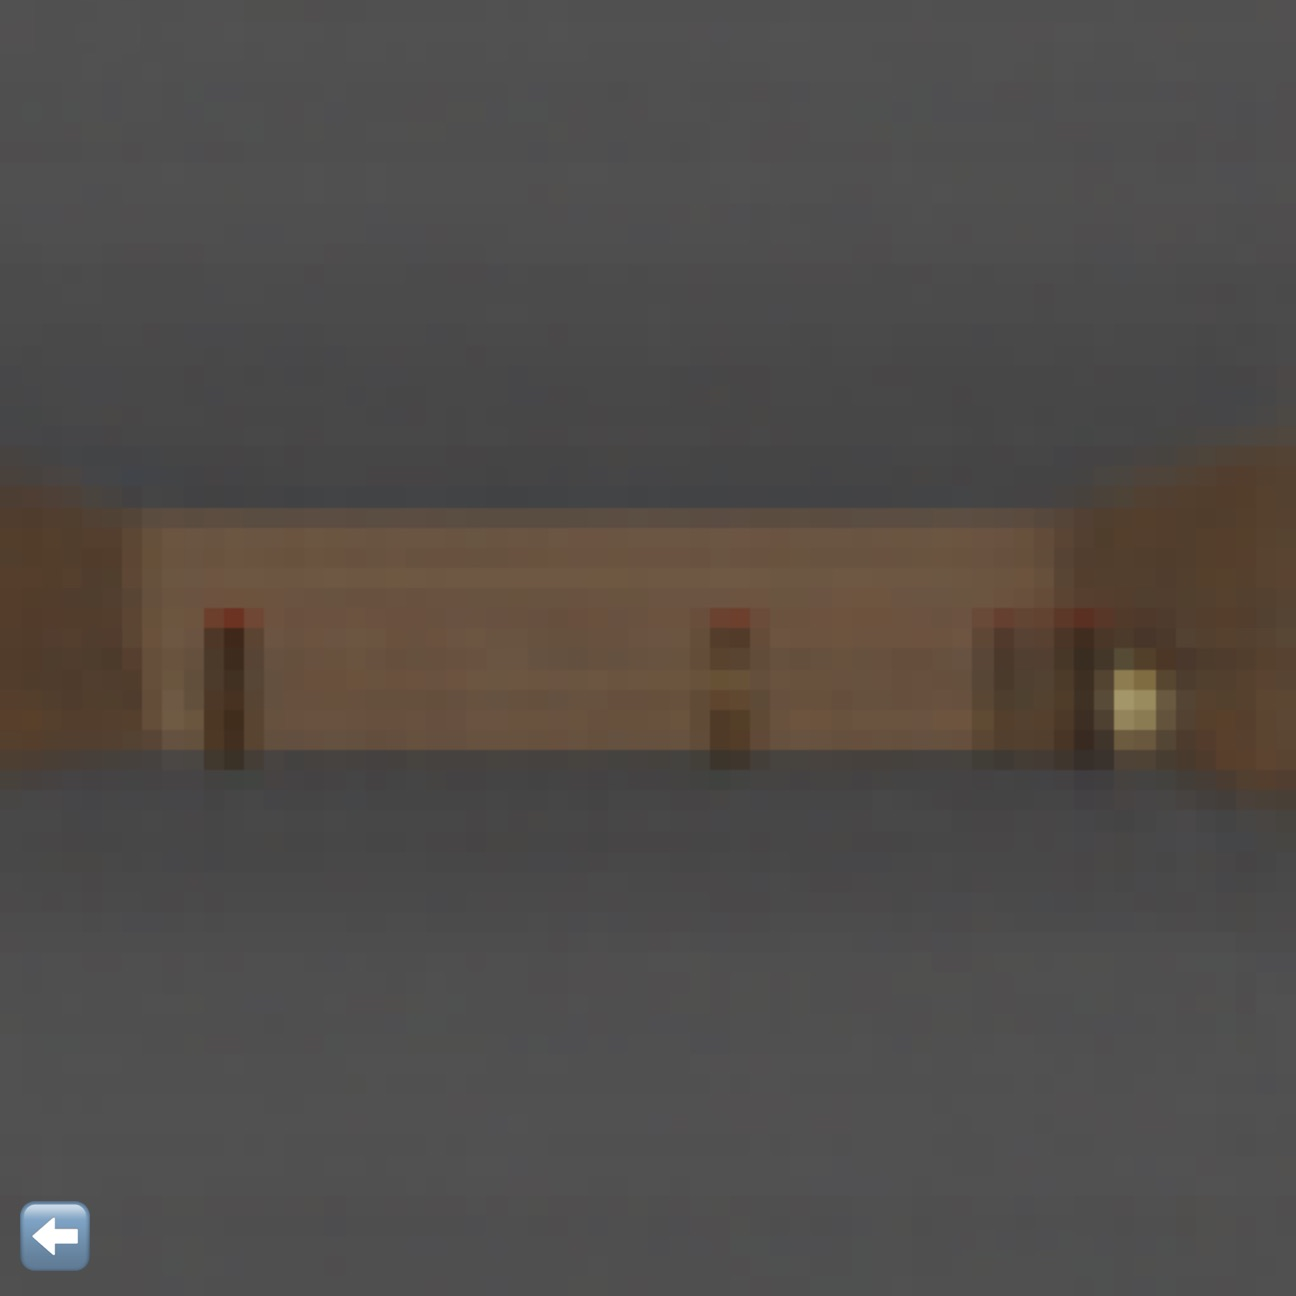
\includegraphics[width=1.0\columnwidth]{demo/demo_doom_adversarial.jpeg}}
\vskip -0.05in
\caption{智能体发现一种对抗性策略，可在某些 rollout 中自动扑灭已经发射的火球。}
\end{center}
\vskip -0.20in
\end{figure}

这一弱点也许解释了为什么许多已有工作虽然学习 RL 环境的动力学模型，却并不完全用这些模型替代真实环境\cite{action_conditional_video_prediction,recurrent_env_sim}。在 \cite{s05_making_the_world_differentiable,s05a_cm,s05b_rl} 提出的 M 模型中，动力学模型是确定性的；若模型并不完美，就容易被智能体利用。PILCO~\cite{pilco} 等贝叶斯模型通过不确定性估计在一定程度上缓解了这个问题，但并未完全解决。近期工作\cite{Nagabandi2017} 将基于模型方法与传统无模型 RL 训练结合，先用学习到的策略初始化策略网络，再依靠无模型方法在真实环境中微调策略。

在 \textit{Learning to Think}~\cite{learning_to_think} 中，RNN M 并不一定总是可靠的预测器。原则上，一个（可能基于进化训练的）RNN C 可以学会忽略有缺陷的 M，也可以利用 M 中某些有用部分来执行任意计算，包括层级规划等。不过，本文并未采用这种做法。我们当前的方法仍更接近早期系统\cite{s05_making_the_world_differentiable,s05a_cm,s05b_rl}，即使用 RNN M 逐步预测并向前规划。不同之处在于，我们像 \textit{Learning to Think} 一样用进化方法训练 C，而不是把传统 RL 与 RNN 结合；这样做更简单，也更通用。

为了让 C 更难利用 M 的缺陷，我们选择用 MDN-RNN 作为动力学模型，使其建模真实环境中可能结果的\textit{分布}，而不是只预测确定性未来。即使真实环境本身是确定性的，MDN-RNN 实际上也会把它近似为随机环境。这样做的好处是，可以在任意环境的更随机版本中训练 C；我们只需调节温度参数 $\tau$，就能控制 M 中随机性的大小，从而在真实性与可利用性之间做权衡。

由于 VAE 编码出的潜在空间本身只是一个对角高斯分布，用高斯混合模型看起来似乎有些复杂。但混合密度模型中的离散模态对包含随机离散事件的环境很有用，例如怪物决定发射火球还是停在原地。单个对角高斯也许足以编码单帧图像，但带混合密度输出层的 RNN 更容易刻画复杂环境背后的逻辑，尤其是包含离散随机状态时。

例如，如果把温度设为很低的 $\tau=0.1$，就相当于用一个几乎确定性的 LSTM 作为 M 来训练 C。在这种梦境环境中，由于模态崩塌，怪物无论面对智能体的何种动作都不会发射火球。M 无法\textit{跳转}到高斯混合模型中“火球形成并发射”的另一种模态。在这样的梦中学到的策略，大多数时候都能获得 2100 的满分；但一旦部署到真实世界，显然会失败，甚至不如随机策略。

再次强调，\textit{Learning to Think} 中更简单、更稳健的做法，并不要求 M 被逐步用于显式规划。C 可以学习把 M 的\textit{子例程}（即 M 权重矩阵的一部分）用于任意计算；当 M 无用且忽略 M 能带来更好表现时，C 也可以学会忽略它。尽管如此，在本文当前的 C--M 变体中，M 的预测仍是训练 C 的关键信号，这更接近早期 C--M 系统~\cite{s05_making_the_world_differentiable,s05a_cm,s05b_rl}，只是结合了进化或黑盒优化。

把温度 $\tau$ 作为 M 的可调参数后，我们可以观察 C 在不同不确定性水平的幻觉环境中训练后的效果，以及这些策略迁移到真实环境后的表现。我们改变虚拟环境温度，在给定温度下训练智能体，然后统计其在真实环境中 100 次随机 rollout 的平均得分：

\begin{table}[ht]
\label{doom_virtual_table}
\vskip -0.0in
\begin{center}
\begin{small}
\begin{sc}
\begin{tabular}{llll}
\toprule
温度$\tau$ &虚拟分数&实际得分\\
\midrule
0.10 & 2086 $\pm$ 140 & 193 $\pm$ 58 \\
0.50 & 2060 $\pm$ 277 & 196 $\pm$ 50 \\
1.00 & 1145 $\pm$ 690 & 868 $\pm$ 511 \\
1.15 & 918 $\pm$ 546 & 1092 $\pm$ 556 \\
1.30 & 732 $\pm$ 269 & 753 $\pm$ 139 \\
\midrule
随机策略& N/A & $210 \pm 108$ \\
Gym 排行榜最优& N/A & $820 \pm 58$ \\
\bottomrule
\end{tabular}
\end{sc}
\end{small}
\end{center}
\vskip -0.1in
\caption{\textit{Take Cover} 在不同温度设置下得分。}
\vskip -0.1in
\end{table}

可以看到，提高 M 的温度会让 C 更难找到对抗性策略；但温度过高又会让虚拟环境过难，导致智能体学不到有效行为。因此，温度实际上是一个需要调节的超参数。温度也会影响智能体发现的策略类型。例如，$\tau=1.15$ 时取得最高得分 $1092\pm556$；将 $\tau$ 进一步提高到 1.30 后，得分降低，但回报方差也更小，策略风险更低。作为比较，OpenAI Gym 排行榜上的最好分数~\cite{takecover} 为 $820 \pm 58$。
\vskip -0.1in
\section{迭代训练程序}

在本文实验中，任务相对简单，因此可以用随机策略收集的数据集训练出合理的世界模型。但如果环境更复杂，会发生什么？在许多困难环境中，只有当智能体学会如何有策略地探索世界后，某些区域才会被观察到。

对于更复杂的任务，需要使用迭代训练程序。智能体必须能够探索世界，并持续收集新观测，使世界模型随时间逐步改进和细化。一个迭代训练流程\cite{learning_to_think} 如下：

\begin{enumerate}
 \item 用随机模型参数初始化 M 和 C。
 \item 在真实环境中 rollout $N$ 次。保存 rollout 过程中的所有动作 $a_t$ 和观测 $x_t$。
 \item 训练 M 建模 $P(x_{t+1}, r_{t+1}, a_{t+1}, d_{t+1} | x_t, a_t, h_t)$，并在 M 内训练 C 以优化期望奖励。
 \item 如果任务尚未完成，回到步骤(2)。
\end{enumerate}

我们已经展示，该训练循环的一次迭代足以解决简单任务。对于更困难的任务，步骤(2)中的控制器需要主动探索那些有助于改进世界模型的环境区域。一个有价值的研究方向，是将人工好奇心、内在动机~\cite{schmidhuber_creativity,s07_intrinsic,s08_curiousity,pathak2017,intrinsic_motivation} 和信息寻求~\cite{SchmidhuberStorck:94,Gottlieb2013} 纳入智能体，以鼓励新颖探索~\cite{Lehman2011}。特别地，可以根据压缩质量的提升来增强奖励函数~\cite{schmidhuber_creativity,s07_intrinsic,s08_curiousity,learning_to_think}。

在当前方法中，M 是一个建模下一帧概率分布的 MDN-RNN。如果它预测得很差，说明智能体遇到了自己尚不熟悉的世界区域。因此，可以改造并复用 M 的训练损失来鼓励好奇心：在真实环境中反转 M 损失函数的符号，就会鼓励智能体探索其不熟悉的区域。由此收集的新数据可能进一步改善世界模型。

迭代训练程序要求 M 不仅预测下一观测 $x$ 和 $done$，还要预测下一时间步的动作和奖励。对于更困难的任务，这可能是必要的。例如，如果智能体需要学习复杂运动技能才能在环境中移动，世界模型会学会模仿已经掌握行走能力的 C 模型。当行走等困难运动技能被吸收到容量更大的世界模型中后，小型 C 模型就可以依赖世界模型已吸收的运动技能，转而专注于学习更高层次的导航能力。

\begin{figure}[ht]
\vskip -0.0in
\begin{center}
\centerline{\includegraphics[width=1.0\columnwidth]{svg/memory_consolidation.pdf}}
\caption{信息如何成为记忆。}
\vskip -0.1in
\end{center}
\vskip -0.2in
\end{figure}

与神经科学文献的一个有趣联系是海马回放研究：动物休息或睡眠时，大脑会重放近期经验。近期经验重放在记忆巩固中发挥重要作用~\cite{Foster2017}，使原本依赖海马的记忆逐渐变得不再依赖海马。正如 \cite{Foster2017} 所说，重放“与其说像做梦，不如说像思考”。关于重放的神经科学视角及其与理论强化学习的联系，可参见 \textit{Replay Comes of Age}~\cite{Foster2017}。

迭代训练可能使 C--M 模型发展出自然的层级学习方式。近期关于 RL 自博弈的工作\cite{asymmetric_self_play,competitive_self_play,continuous_adaptation_via_meta_learning} 以及 PowerPlay\cite{s10_powerplay,s11_powerplay} 也在探索能够产生自然课程学习的方法\cite{s09_optimal_order}。我们认为这是强化学习中很值得继续研究的方向之一。

\section{相关工作}

关于学习动力学模型并用该模型训练策略，已有大量文献。许多概念最早在 1980 年代的前馈神经网络(FNN)研究\cite{Werbos87specifications,Munro87,RobinsonFallside89,Werbos89identification,NguyenWidrow89} 和 1990 年代的 RNN 研究\cite{s05_making_the_world_differentiable,s05a_cm,s05b_rl,s05c_boredom} 中得到探索，并为 \textit{Learning to Think}~\cite{learning_to_think} 奠定了部分基础。较近的 PILCO~\cite{pilco,pilco_tutorial,McAllister2017} 是一种基于概率模型的策略搜索方法，用于解决困难控制问题。PILCO 使用从环境收集的数据，以高斯过程(GP)模型学习系统动力学，再利用该模型采样大量轨迹，从而训练控制器完成摆杆或骑独轮车等任务。

\begin{figure}[ht]
\vskip -0.05in
\begin{center}
\centerline{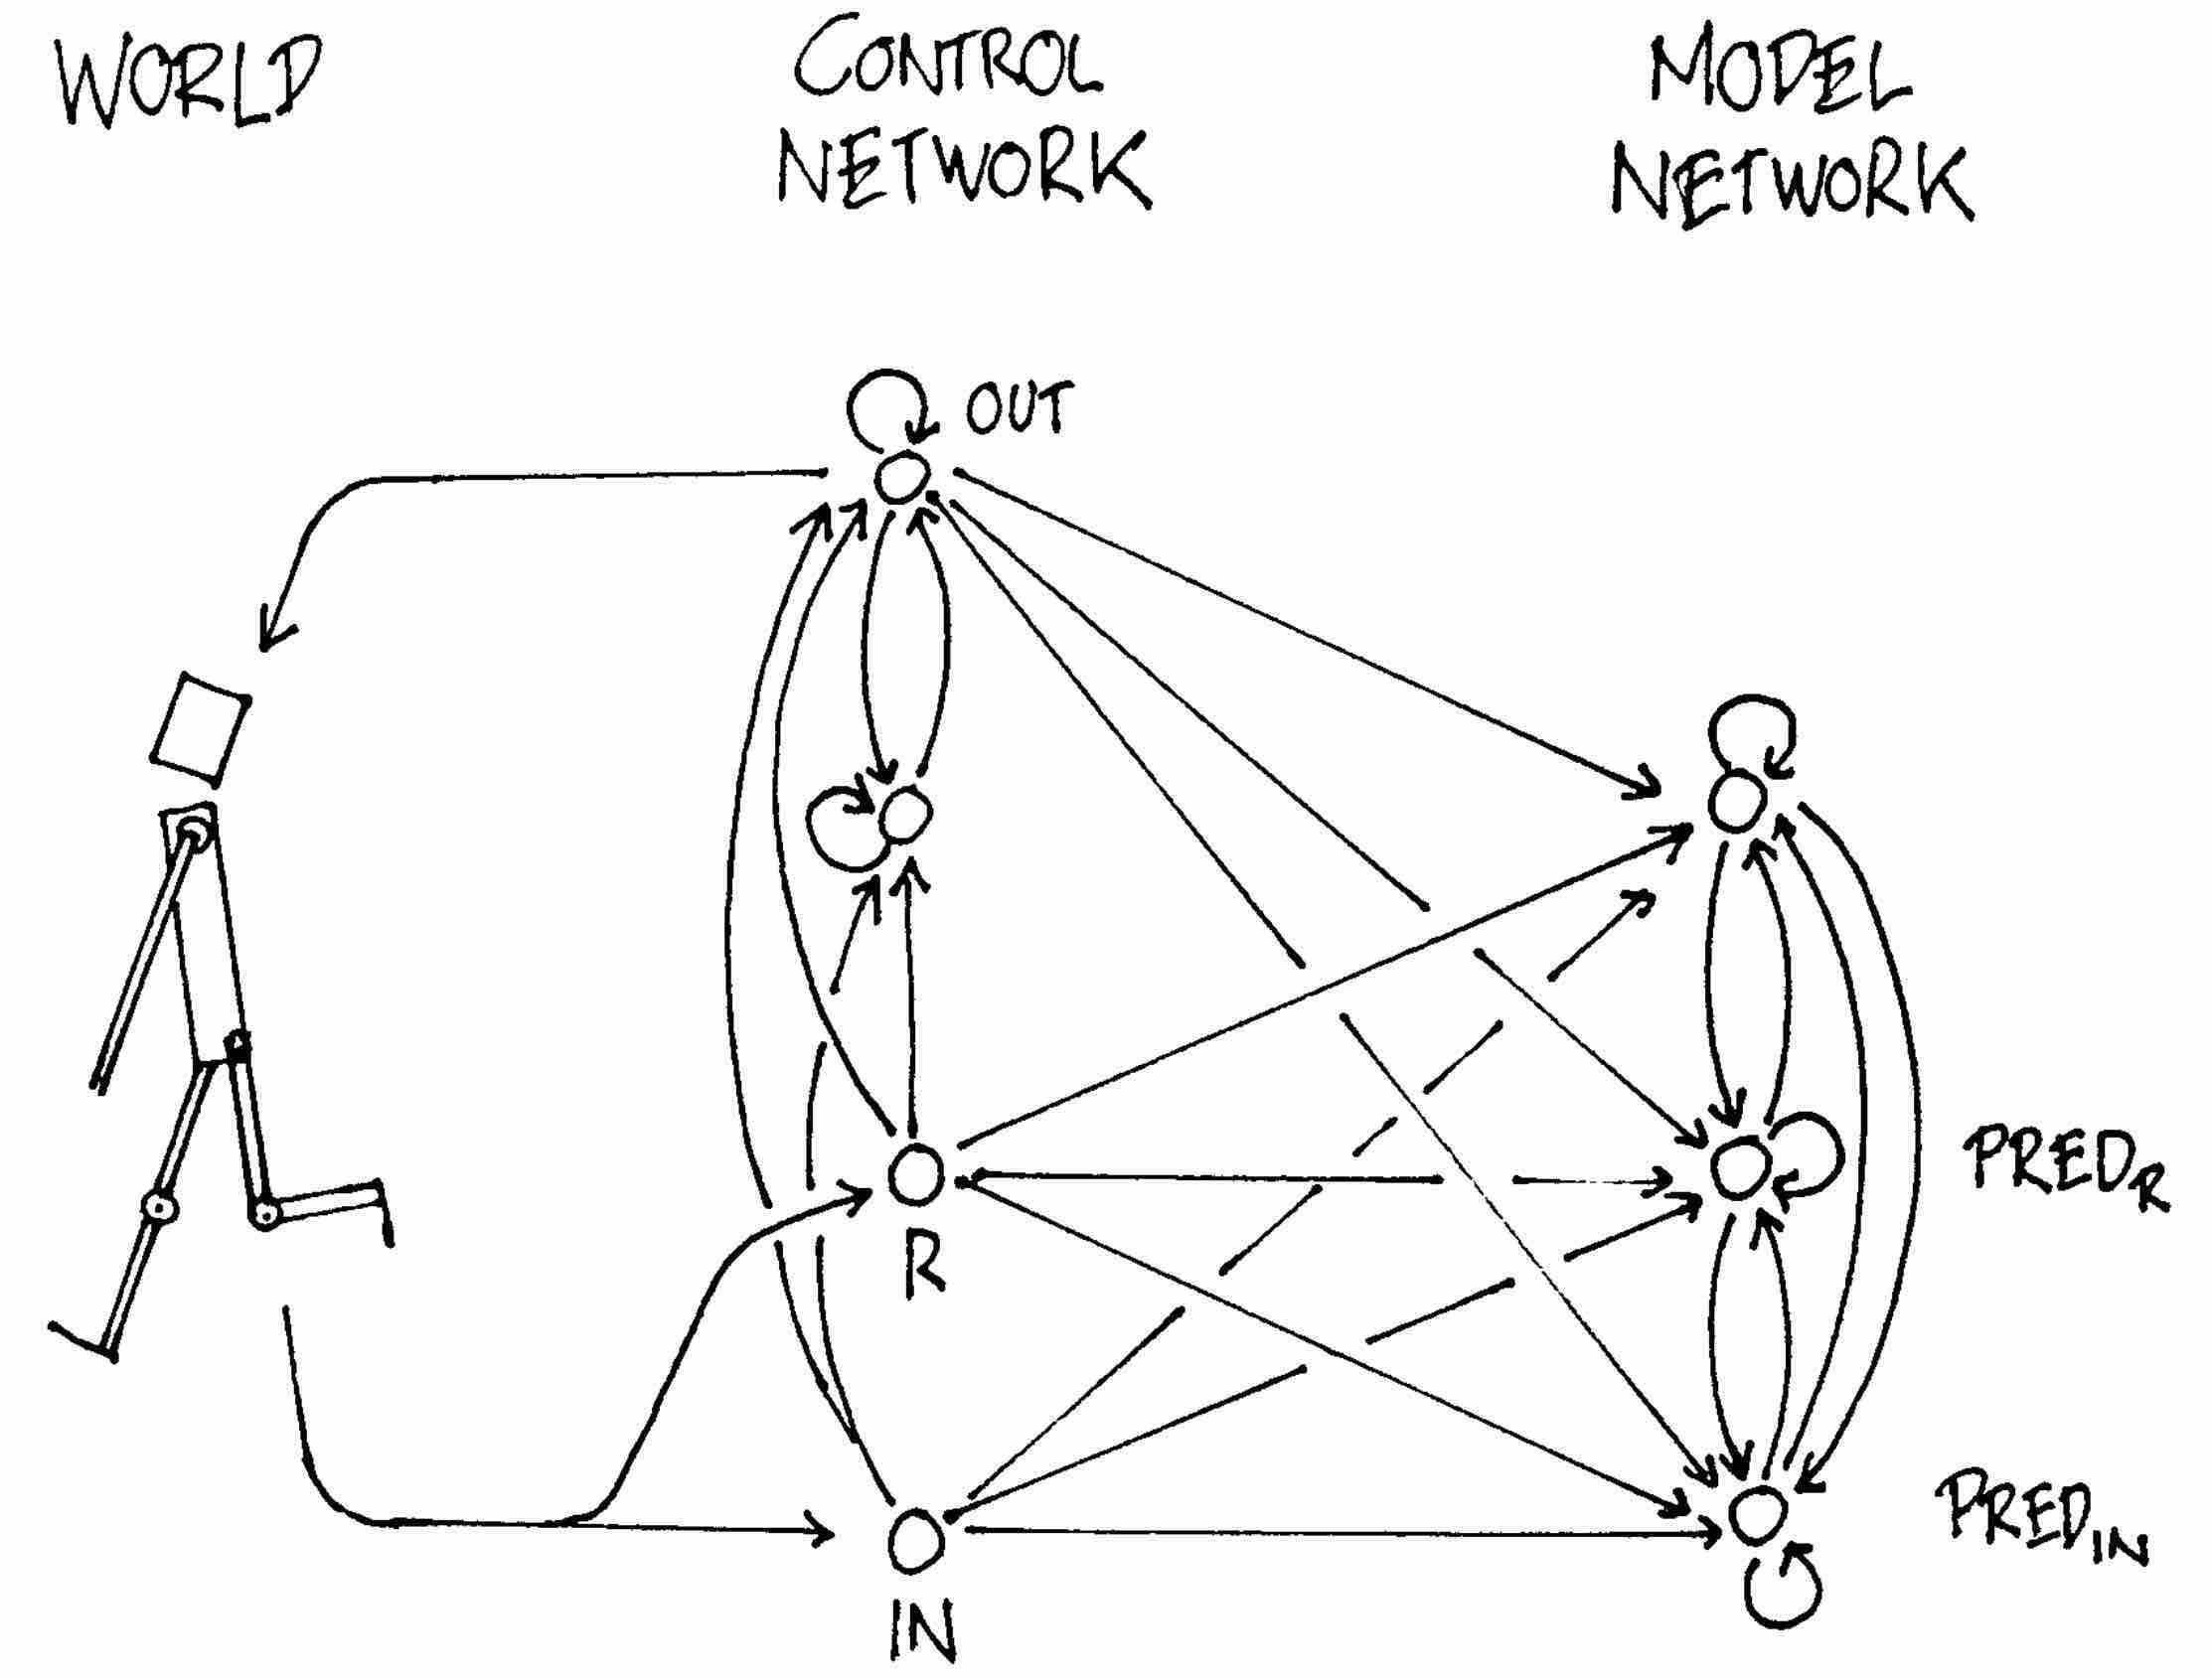
\includegraphics[width=1.0\columnwidth]{assets/world_models_1990.jpeg}}
\vskip -0.10in
\caption{带世界 RNN 内部模型的控制器\cite{s05_making_the_world_differentiable}。}
\end{center}
\vskip -0.25in
\end{figure}

高斯过程在小规模低维数据上效果良好，但其计算复杂度使其难以扩展到大量高维观测历史。近期另一些工作\cite{deep_pilco,Depeweg2017} 使用贝叶斯神经网络而非 GP 来学习动力学模型。这些方法在若干挑战性控制任务上取得了有希望的结果\cite{Hein2017}，但这些任务中的状态通常已知且定义良好，观测维度也相对较低。本文关注的是从高维视觉数据中建模动力学，输入是一串原始像素帧。

在机器人控制中，仅从相机视频输入学习系统动力学是一个困难但重要的问题。早期主动视觉 RL 工作训练 FNN 用视频序列当前帧预测下一帧\cite{s04_trajectories}，并利用该预测模型训练一个移动中央凹的控制网络，在视觉场景中寻找目标。为避免直接从高维像素图像学习动力学带来的困难，研究者尝试先用神经网络学习视频帧的压缩表示。沿这一方向的工作\cite{learning_deep_dynamical_models_from_image_pixels,from_pixels_to_torques} 使用自动编码器瓶颈层作为低维特征向量，从像素输入控制摆杆。从压缩潜在空间学习动力学模型，可以显著提高 RL 算法的数据效率\cite{deep_spacial_autoencoders,embed_to_control,finn_lecture}。更多内容可参考 Finn 关于基于模型 RL 的讲座\cite{finn_lecture}。

电子游戏环境也常被用作基于模型 RL 的试验场。\cite{game_engine_learning} 使用前馈卷积神经网络(CNN)学习电子游戏的前向模拟模型。对游戏智能体而言，预测不同动作如何影响环境未来状态很有用：如果智能体能根据当前状态和动作预测未来，就可以选择最符合目标的动作。早期工作\cite{NguyenWidrow89,s04_trajectories} 已经展示了这一点（当时计算成本比今天高得多），近期在若干竞争性 VizDoom 环境中的研究\cite{learn_to_act_by_predicting_future} 也给出了类似结果。

上述工作多使用 FNN 预测下一视频帧。若要捕捉更长期的时间依赖，则需要序列建模能力更强的模型。RNN 是适合序列建模的强大模型\cite{graves_rnn}。在题为 \textit{Hallucination with RNNs} 的讲座中\cite{graves_lecture}，Graves 展示了 RNN 学习 Atari 游戏环境概率模型的能力：训练后的 RNN 能学习游戏结构，并自行生成类似游戏关卡的幻觉。

使用 RNN 构建内部模型并据此推理未来的思想，早在 1990 年的 \textit{Making the World Differentiable}~\cite{s05_making_the_world_differentiable} 中就已出现，并在后续工作\cite{s05a_cm,s05b_rl,s05c_boredom} 中继续发展。较近的 \textit{Learning to Think}~\cite{learning_to_think} 提出了一个统一框架，用于构建基于 RNN 的通用问题求解器：它能够学习环境的世界模型，并利用该模型推理未来。后续工作也使用基于 RNN 的模型生成未来多帧~\cite{recurrent_env_sim,action_conditional_video_prediction,Denton2017}，或将其作为推理未来的内部模型\cite{Silver2016,imagination_agent,Watters2017}。

本文使用进化策略训练控制器，因为它有若干实际优点。例如，我们只需要向优化器提供最终累积奖励，而不必提供完整历史。ES 也易于并行化：可以在多个 worker 上用不同候选解启动许多 \texttt{rollout} 实例，并快速并行计算一组累积奖励。近期工作\cite{pathnet,openai,stablees,stanley2017} 已经表明，在许多强基线上，ES 是传统深度 RL 方法的可行替代方案。

在深度 RL 方法流行之前\cite{dqn}，基于进化的算法就已被证明能够有效解决 RL 任务~\cite{neat,gom5_ne_accelerated,gom2_coevolve,hyperneat,pepg,evolving_neural_networks}。进化算法甚至可以从高维像素输入解决困难 RL 任务~\cite{kou1_torcs,hausknecht,parker2012}。近期工作\cite{vae_evolution} 将 VAE 与 ES 结合，与本文方法相近。

\section{讨论}

\begin{figure}[ht]
\vskip -0.05in
\begin{center}
\centerline{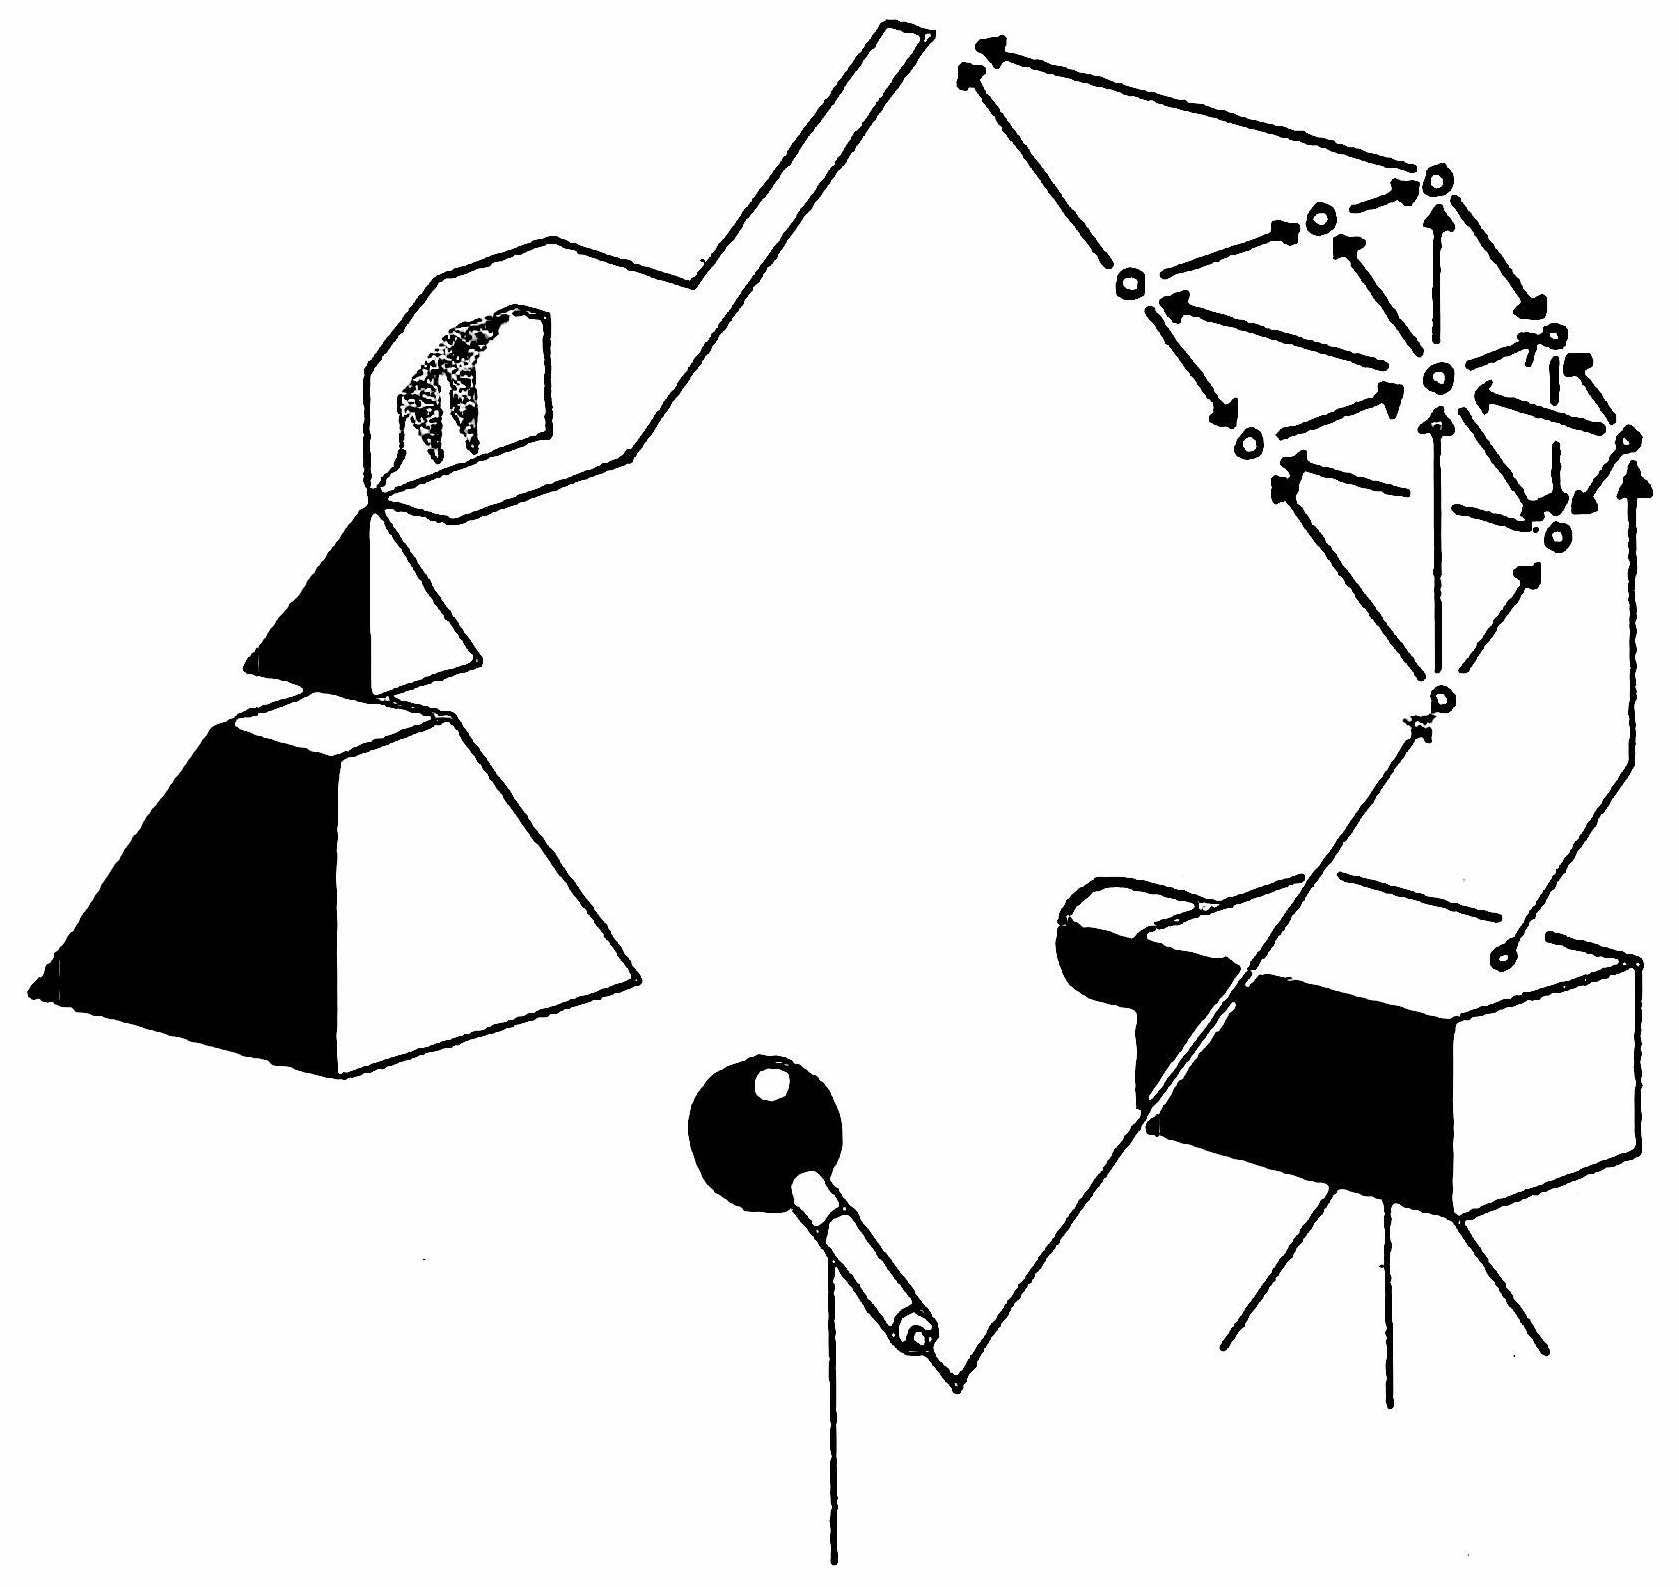
\includegraphics[width=1.0\columnwidth]{assets/world_models_1990_feedback.jpeg}}
\caption{1990 年关于基于 RNN 的控制器与环境交互的早期示意图\cite{s05_making_the_world_differentiable}。}
\vskip -0.15in
\end{center}
\vskip -0.1in
\end{figure}

我们已经证明，智能体可以完全在其模拟的潜在空间梦境世界中学习任务。这种做法有若干实际好处。例如，运行计算密集型游戏引擎需要大量计算资源来把游戏状态渲染成图像帧，或计算与当前游戏目标无直接关系的物理过程。与其在真实环境中反复训练智能体，我们可以在模拟环境中任意多次训练。现实世界中的训练成本更高，因此，逐步训练出能够模拟现实的世界模型，可能有助于把策略迁移回真实世界。本文方法也可以作为 sim2real 方法\cite{Bousmalis2017,Higgins2017} 的补充。

此外，可以利用深度学习框架，在分布式环境中用 GPU 加速世界模型模拟。把世界模型实现为完全可微的循环计算图，还有一个潜在好处：我们或许可以直接使用反向传播在梦境中训练智能体，微调其策略以最大化目标函数\cite{s05_making_the_world_differentiable,s05a_cm,s05b_rl}。

将 V 模型实现为 VAE 并单独训练也有局限，因为它可能编码与任务无关的观测信息。无监督学习本身并不知道哪些内容对当前任务有用。例如，VAE 在 Doom 环境中会复现侧墙上并不重要的砖块纹理，却可能无法复现 CarRacing 中与任务相关的赛道格子。如果把 VAE 与预测奖励的 M 模型联合训练，它也许会更关注图像中与任务相关的区域；但代价是，该 VAE 可能难以在不重新训练的情况下有效复用于新任务。

学习任务相关特征也与神经科学有关。初级感觉神经元在获得奖励后会解除抑制，这表明至少在成年阶段，它们更倾向于学习与任务相关的特征，而不是任意特征~\cite{Pi2013}。

%Future work might explore the use of an unsupervised segmentation layer like in ~\cite{Byravan2017} to extract better feature representations that might be more useful and interpretable compared to the VAE representations learned.

另一个问题是世界模型容量有限。现代存储设备可以保存迭代训练过程中产生的大量历史数据，但基于 LSTM~\cite{lstm,s12_lstm_forget} 的世界模型未必能把所有记录信息都存入权重连接中。人脑可以以某种分辨率保存几十年甚至更久的记忆\cite{brain_capacity}；而用反向传播训练的神经网络容量有限，并会遭遇灾难性遗忘等问题\cite{Ratcliff1990,French1994,Kirkpatrick2016}。如果希望智能体学会探索更复杂的世界，后续工作可以考虑用容量更高的模型替代小型 MDN-RNN~\cite{outrageously_large_neural_nets,hypernetworks,suarez2017,wavenet,attention}，或引入外部记忆模块~\cite{Gemici2017}。

类似早期基于 RNN 的 C--M 系统~\cite{s05_making_the_world_differentiable,s05a_cm,s05b_rl,s05c_boredom}，本文系统逐时间步模拟可能未来，并未利用类似人类的层级规划或抽象推理；后者通常会忽略无关的时空细节。\textit{Learning to Think}~\cite{learning_to_think} 并不局限于这种朴素方式。它允许循环 C 学习调用循环 M 的\textit{子例程}，并以任意可计算方式复用这些子例程来求解问题，例如进行层级规划，或利用 M 中类似程序的权重矩阵。\textit{One Big Net}~\cite{onebignet2018} 是 C--M 方法的一个扩展，将 C 和 M 合并为单个网络，并使用类似 PowerPlay~\cite{s10_powerplay,s11_powerplay} 的行为回放机制（即把教师网络行为压缩到学生网络中~\cite{chunker91and92}），以便在学习新的预测和控制技能时避免遗忘旧技能。

\section*{鸣谢}

感谢 Blake Richards、Kai Arulkumaran、Ankur Handa、Kory Mathewson、Kyle McDonald、Denny Britz、Elwin Ha 和 Natasha Jaques 对本文提供认真反馈，并从各自技术领域给出宝贵观点和见解。

本文交互式在线版本使用 \url{distill.pub} 的网页技术构建。感谢 Chris Olah 和 Distill 编辑团队其他成员提供宝贵反馈与慷慨的编辑支持，并支持我们使用 Distill 技术。

\url{worldmodels.github.io} 上的交互式演示全部使用 \texttt{p5.js} 构建。得益于 \texttt{deeplearn.js}，这些机器学习模型可以部署在网页浏览器中；\texttt{deeplearn.js} 是 Google \textit{People+AI Research Initiative} (PAIR) 团队开发的浏览器端硬件加速机器学习框架。特别感谢 Nikhil Thorat 和 Daniel Smilkov 在开发过程中的帮助。

感谢 Alex Graves、Douglas Eck、Mike Schuster、Rajat Monga、Vincent Vanhoucke、Jeff Dean 和 Google Brain 团队提供有益反馈，并鼓励我们探索这一研究方向。实验在 Google Cloud Platform 提供的 Ubuntu 虚拟机上完成。文中若有错误，责任均由作者承担，并不代表审稿人和同事的观点。

%

%\section*{Citation}

%For attribution in academic contexts, cite this work as:

%\texttt{Ha and Schmidhuber, World Models, 2018.} %\url{https://doi.org/10.5281/zenodo.1207631}

%\medskip

%\textit{BibTeX} Citation:

%\begin{verbatim}
%@article{Ha2018WorldModels,
% author = {Ha, D. and Schmidhuber, J.},
% title = {World Models},
% eprint = {arXiv:1803.10122},
% doi = {10.5281/zenodo.1207631},
% url = {https://worldmodels.github.io},
% year = {2018}
%}
%\end{verbatim}

%\begin{figure}[ht]

%\begin{center}
%\centerline{\includegraphics[width=1.0\columnwidth]{svg/bibtex_citation_text.pdf}}
%\end{center}
%\vskip -0.45in
%\end{figure}

\appendix
\section{附录}

本节进一步说明本文使用的模型结构和训练方法。

\subsection{变分自编码器}

\begin{figure}[ht]
\vskip -0.10in
\begin{center}
\centerline{\includegraphics[width=0.5\columnwidth]{svg/conv_vae_label.pdf}}
\vskip -0.15in
\caption{ConvVAE 各层张量形状示意。}
\end{center}
\vskip -0.30in
\end{figure}

我们训练了一个卷积变分自编码器（ConvVAE），作为智能体的 V 模型。与普通自编码器相比，在潜变量 $z$ 上施加高斯先验会限制每一帧可被压缩进潜表示的信息量；同时，这一先验也使世界模型对 M 模型生成的不真实 $z$ 向量更为稳健。

环境给出的观测可能是高维像素图像，因此我们先将每张图像缩放到 $64\times64$ 像素，并把缩放后的图像作为 V 模型的输入。每个像素由 0 到 1 之间的三个浮点数表示，对应 RGB 三个通道。ConvVAE 接收 $64\times64\times3$ 的输入张量，并通过 4 个卷积层将其编码为低维向量 $\mu$ 和 $\sigma$，二者的维度均为 $N_z$。潜变量 $z$ 从高斯分布 $N(\mu, \sigma I)$ 中采样得到。在 CarRacing 任务中，$N_z=32$；在 Doom 任务中，$N_z=64$。随后，潜变量 $z$ 经过 4 个反卷积层，用于解码并重建图像。

每个卷积层和反卷积层的步幅均为 2。图中以\textit{斜体}标注各层，格式为\textit{激活类型 输出通道数 x 滤波器大小}。除输出层外，所有卷积层和反卷积层都使用 ReLU 激活函数；输出层需要把像素值限制在 0 到 1 之间，因此不采用相同设置。我们使用随机策略收集的数据训练该模型 1 个 epoch，优化目标包括 KL 损失，以及输入图像与重建图像之间的 $L^2$ 距离所定义的重建损失。

\subsection{循环神经网络}

对于 M 模型，我们采用 LSTM~\cite{lstm} 循环神经网络，并使用混合密度网络（Mixture Density Network, MDN）~\cite{bishop} 作为输出层。该网络用于把下一时刻的 $z$ 的概率分布建模为高斯混合分布。这一做法与 \cite{graves_rnn} 中无条件手写生成部分，以及 SketchRNN~\cite{sketchrnn} 中仅含解码器的设置相近。主要区别在于，我们没有建模 $z$ 各元素之间的相关系数，而是让 MDN-RNN 输出因子化高斯分布的对角协方差矩阵。

\begin{figure}[ht]
\vskip -0.05in
\begin{center}
\centerline{\includegraphics[width=1.0\columnwidth]{svg/mdn_rnn.pdf}}
\vskip -0.00in
\caption{与 \cite{graves_rnn,sketchrnn} 类似的 MDN-RNN 解码器。}
\end{center}
\vskip -0.35in
\end{figure}

不同于手写和草图生成工作中用 MDN-RNN 建模下一笔画的概率密度，我们建模的是下一时刻潜变量 $z$ 的概率密度。生成虚拟环境时，我们在每个时间步从该分布中采样。在 Doom 任务中，我们还使用 MDN-RNN 预测智能体是否会在当前帧死亡。当该概率超过 50\% 时，虚拟环境中的 \textit{done} 被设为 \textit{true}。由于死亡在单个时间步内属于低概率事件，我们发现这种阈值截断方式比从伯努利分布中直接采样更稳定。

MDN-RNN 使用随机策略智能体收集的数据训练 20 个 epoch。在 CarRacing 任务中，LSTM 使用 256 个隐藏单元；在 Doom 任务中，LSTM 使用 512 个隐藏单元。两个任务均采用 5 个高斯混合分量，并且不建模相关系数 $\rho$，因此 $z$ 从因子化高斯混合分布中采样。

使用记录数据对 MDN-RNN 进行 teacher forcing 训练时，我们为每一帧存储预先计算好的 $\mu$ 和 $\sigma$。每次构造训练批次时，再采样输入 $z \sim N(\mu, \sigma)$，以避免 MDN-RNN 过拟合到某一次特定采样得到的 $z$。

\subsection{控制器}

在两个环境中，我们都使用 $\tanh$ 非线性函数对动作空间进行裁剪和约束，使其落在合适范围内。例如，在 CarRacing 任务中，方向盘取值范围为 -1 到 1，油门为 0 到 1，刹车也为 0 到 1。在 Doom 环境中，我们把离散动作转换为 -1 到 1 之间的连续动作空间，并将该区间划分为三段，分别表示智能体向左移动、保持原位或向右移动。C 模型的输入是一个特征向量，由 $z$ 和 MDN-RNN 的隐藏状态组成。在 CarRacing 任务中，该隐藏状态为 LSTM 的输出向量 $h$；在 Doom 任务中，则同时使用 LSTM 的记忆单元向量 $c$ 和输出向量 $h$。

\subsection{进化策略}

我们使用\textit{协方差矩阵自适应进化策略}（Covariance-Matrix Adaptation Evolution Strategy, CMA-ES）~\cite{cmaes} 来优化 C 模型的权重。按照 \textit{Evolving Stable Strategies}~\cite{stablees} 的做法，我们设定种群大小为 64，并让每个智能体在不同初始随机种子下执行任务 16 次。智能体的适应度定义为 16 次随机 rollout 的\textit{平均累计奖励}。下图给出了每一代 64 个智能体中最佳个体、最差个体以及种群平均适应度的变化：

\begin{figure}[ht]
\vskip -0.00in
\begin{center}
\centerline{\includegraphics[width=1.0\columnwidth]{svg/carracing.pdf}}
\vskip -0.15in
\caption{训练\texttt{CarRacing-v0}}
\end{center}
\vskip -0.25in
\end{figure}

该环境的通过条件是智能体在 100 个随机 rollout 上的平均得分超过 900。因此，我们每隔 25 代取当前表现最好的智能体，并在 1024 个随机 rollout 场景上进行评估，用红线记录其平均得分。训练到第 1800 代后，一个智能体在 1024 个随机 rollout 上取得了 900.46 的平均得分。我们之所以使用 1024 次 rollout 而不是 100 次，是因为 64 核机器上的每个进程已经配置为运行 16 次，相当于每 25 代额外使用整整一代计算来评估当前最佳智能体 1024 次。下图展示了同一智能体在 100 次 rollout 上的评估结果：

\begin{figure}[ht]
\vskip -0.05in
\begin{center}
\centerline{\includegraphics[width=1.0\columnwidth]{svg/carracing_histogram.pdf}}
\vskip -0.10in
\caption{累计奖励的直方图，得分906$\pm$ 21.}
\end{center}
\vskip -0.4in
\end{figure}

我们还测试了一类只能访问 VAE 输出的 $z$ 向量、不能访问 RNN 隐藏状态的智能体。具体来说，我们尝试了两个变体：第一个变体中，C 模型直接将 $z$ 映射到动作空间 $a$；第二个变体在 $z$ 与 $a$ 之间加入一个包含 40 个 $\tanh$ 激活单元的隐藏层，将 C 模型的参数量增加到 1443，使其与原始设置更具可比性。

\begin{figure}[ht]
\vskip -0.05in
\begin{center}
\centerline{\includegraphics[width=1.0\columnwidth]{svg/carracing_histogram_z.pdf}}
\vskip -0.10in
\caption{当智能体只看到$z_t$,得分为632$\pm$ 251.}
\end{center}
\vskip -0.4in
\end{figure}

\begin{figure}[ht]
\vskip -0.05in
\begin{center}
\centerline{\includegraphics[width=1.0\columnwidth]{svg/carracing_histogram_z_hidden.pdf}}
\vskip -0.10in
\caption{当智能体只看到 $z_t$ 且使用隐藏层时，得分为 788 $\pm$ 141。}
\end{center}
\vskip -0.4in
\end{figure}

\subsection{DoomRNN}

我们在称为 \textit{DoomRNN} 的虚拟 Doom 环境中进行了类似实验。需要说明的是，我们并没有尝试在真实 VizDoom 环境中训练智能体；VizDoom 只用于通过随机策略收集训练数据。与 VizDoom 相比，\textit{DoomRNN} 的计算效率更高，因为它只在潜空间中运行，不需要在每个时间步渲染屏幕截图，也不需要运行真实的 Doom 游戏引擎。

\begin{figure}[ht]
\vskip -0.05in
\begin{center}
\centerline{\includegraphics[width=1.0\columnwidth]{svg/doomrnn.pdf}}
\vskip -0.05in
\caption{训练DoomRNN。}
\end{center}
\vskip -0.2in
\end{figure}

在构造的虚拟 DoomRNN 环境中，我们略微提高采样温度，使用 $\tau=1.15$，让智能体在更具挑战性的环境中学习。最佳智能体在 1024 个随机 rollout 上取得了 959 的平均分（即图中红线的最高点）。将同一智能体部署到真实的 \textit{DoomTakeCover-v0}~\cite{takecover} 环境后，它在 100 个随机 rollout 上取得了 1092 $\pm$ 556 的平均得分。

\begin{figure}[ht]
\vskip -0.00in
\begin{center}
\centerline{\includegraphics[width=0.9\columnwidth]{svg/doomtakecover_histogram.pdf}}
\vskip -0.05in
\caption{在真实 VizDoom 环境中连续 100 次试验的存活时间步数直方图。得分为 1092 $\pm$ 556。}
\end{center}
\vskip -0.2in
\end{figure}

\bibliography{main}
\bibliographystyle{icml2018}

\end{document}
